% Options for packages loaded elsewhere
\PassOptionsToPackage{unicode}{hyperref}
\PassOptionsToPackage{hyphens}{url}
%
\documentclass[
  man]{apa6}
\usepackage{amsmath,amssymb}
\usepackage{lmodern}
\usepackage{iftex}
\ifPDFTeX
  \usepackage[T1]{fontenc}
  \usepackage[utf8]{inputenc}
  \usepackage{textcomp} % provide euro and other symbols
\else % if luatex or xetex
  \usepackage{unicode-math}
  \defaultfontfeatures{Scale=MatchLowercase}
  \defaultfontfeatures[\rmfamily]{Ligatures=TeX,Scale=1}
\fi
% Use upquote if available, for straight quotes in verbatim environments
\IfFileExists{upquote.sty}{\usepackage{upquote}}{}
\IfFileExists{microtype.sty}{% use microtype if available
  \usepackage[]{microtype}
  \UseMicrotypeSet[protrusion]{basicmath} % disable protrusion for tt fonts
}{}
\makeatletter
\@ifundefined{KOMAClassName}{% if non-KOMA class
  \IfFileExists{parskip.sty}{%
    \usepackage{parskip}
  }{% else
    \setlength{\parindent}{0pt}
    \setlength{\parskip}{6pt plus 2pt minus 1pt}}
}{% if KOMA class
  \KOMAoptions{parskip=half}}
\makeatother
\usepackage{xcolor}
\usepackage{graphicx}
\makeatletter
\def\maxwidth{\ifdim\Gin@nat@width>\linewidth\linewidth\else\Gin@nat@width\fi}
\def\maxheight{\ifdim\Gin@nat@height>\textheight\textheight\else\Gin@nat@height\fi}
\makeatother
% Scale images if necessary, so that they will not overflow the page
% margins by default, and it is still possible to overwrite the defaults
% using explicit options in \includegraphics[width, height, ...]{}
\setkeys{Gin}{width=\maxwidth,height=\maxheight,keepaspectratio}
% Set default figure placement to htbp
\makeatletter
\def\fps@figure{htbp}
\makeatother
\setlength{\emergencystretch}{3em} % prevent overfull lines
\providecommand{\tightlist}{%
  \setlength{\itemsep}{0pt}\setlength{\parskip}{0pt}}
\setcounter{secnumdepth}{-\maxdimen} % remove section numbering
% Make \paragraph and \subparagraph free-standing
\ifx\paragraph\undefined\else
  \let\oldparagraph\paragraph
  \renewcommand{\paragraph}[1]{\oldparagraph{#1}\mbox{}}
\fi
\ifx\subparagraph\undefined\else
  \let\oldsubparagraph\subparagraph
  \renewcommand{\subparagraph}[1]{\oldsubparagraph{#1}\mbox{}}
\fi
\newlength{\cslhangindent}
\setlength{\cslhangindent}{1.5em}
\newlength{\csllabelwidth}
\setlength{\csllabelwidth}{3em}
\newlength{\cslentryspacingunit} % times entry-spacing
\setlength{\cslentryspacingunit}{\parskip}
\newenvironment{CSLReferences}[2] % #1 hanging-ident, #2 entry spacing
 {% don't indent paragraphs
  \setlength{\parindent}{0pt}
  % turn on hanging indent if param 1 is 1
  \ifodd #1
  \let\oldpar\par
  \def\par{\hangindent=\cslhangindent\oldpar}
  \fi
  % set entry spacing
  \setlength{\parskip}{#2\cslentryspacingunit}
 }%
 {}
\usepackage{calc}
\newcommand{\CSLBlock}[1]{#1\hfill\break}
\newcommand{\CSLLeftMargin}[1]{\parbox[t]{\csllabelwidth}{#1}}
\newcommand{\CSLRightInline}[1]{\parbox[t]{\linewidth - \csllabelwidth}{#1}\break}
\newcommand{\CSLIndent}[1]{\hspace{\cslhangindent}#1}
\ifLuaTeX
\usepackage[bidi=basic]{babel}
\else
\usepackage[bidi=default]{babel}
\fi
\babelprovide[main,import]{english}
% get rid of language-specific shorthands (see #6817):
\let\LanguageShortHands\languageshorthands
\def\languageshorthands#1{}
% Manuscript styling
\usepackage{upgreek}
\captionsetup{font=singlespacing,justification=justified}

% Table formatting
\usepackage{longtable}
\usepackage{lscape}
% \usepackage[counterclockwise]{rotating}   % Landscape page setup for large tables
\usepackage{multirow}		% Table styling
\usepackage{tabularx}		% Control Column width
\usepackage[flushleft]{threeparttable}	% Allows for three part tables with a specified notes section
\usepackage{threeparttablex}            % Lets threeparttable work with longtable

% Create new environments so endfloat can handle them
% \newenvironment{ltable}
%   {\begin{landscape}\centering\begin{threeparttable}}
%   {\end{threeparttable}\end{landscape}}
\newenvironment{lltable}{\begin{landscape}\centering\begin{ThreePartTable}}{\end{ThreePartTable}\end{landscape}}

% Enables adjusting longtable caption width to table width
% Solution found at http://golatex.de/longtable-mit-caption-so-breit-wie-die-tabelle-t15767.html
\makeatletter
\newcommand\LastLTentrywidth{1em}
\newlength\longtablewidth
\setlength{\longtablewidth}{1in}
\newcommand{\getlongtablewidth}{\begingroup \ifcsname LT@\roman{LT@tables}\endcsname \global\longtablewidth=0pt \renewcommand{\LT@entry}[2]{\global\advance\longtablewidth by ##2\relax\gdef\LastLTentrywidth{##2}}\@nameuse{LT@\roman{LT@tables}} \fi \endgroup}

% \setlength{\parindent}{0.5in}
% \setlength{\parskip}{0pt plus 0pt minus 0pt}

% Overwrite redefinition of paragraph and subparagraph by the default LaTeX template
% See https://github.com/crsh/papaja/issues/292
\makeatletter
\renewcommand{\paragraph}{\@startsection{paragraph}{4}{\parindent}%
  {0\baselineskip \@plus 0.2ex \@minus 0.2ex}%
  {-1em}%
  {\normalfont\normalsize\bfseries\itshape\typesectitle}}

\renewcommand{\subparagraph}[1]{\@startsection{subparagraph}{5}{1em}%
  {0\baselineskip \@plus 0.2ex \@minus 0.2ex}%
  {-\z@\relax}%
  {\normalfont\normalsize\itshape\hspace{\parindent}{#1}\textit{\addperi}}{\relax}}
\makeatother

% \usepackage{etoolbox}
\makeatletter
\patchcmd{\HyOrg@maketitle}
  {\section{\normalfont\normalsize\abstractname}}
  {\section*{\normalfont\normalsize\abstractname}}
  {}{\typeout{Failed to patch abstract.}}
\patchcmd{\HyOrg@maketitle}
  {\section{\protect\normalfont{\@title}}}
  {\section*{\protect\normalfont{\@title}}}
  {}{\typeout{Failed to patch title.}}
\makeatother

\usepackage{xpatch}
\makeatletter
\xapptocmd\appendix
  {\xapptocmd\section
    {\addcontentsline{toc}{section}{\appendixname\ifoneappendix\else~\theappendix\fi\\: #1}}
    {}{\InnerPatchFailed}%
  }
{}{\PatchFailed}
\keywords{body position, motor development, everyday experiences, sitting, machine learning\newline\indent Word count: 11,995}
\DeclareDelayedFloatFlavor{ThreePartTable}{table}
\DeclareDelayedFloatFlavor{lltable}{table}
\DeclareDelayedFloatFlavor*{longtable}{table}
\makeatletter
\renewcommand{\efloat@iwrite}[1]{\immediate\expandafter\protected@write\csname efloat@post#1\endcsname{}}
\makeatother
\usepackage{csquotes}
\raggedbottom
\ifLuaTeX
  \usepackage{selnolig}  % disable illegal ligatures
\fi
\usepackage[style=apa,]{biblatex}
\addbibresource{master.bib}
\IfFileExists{bookmark.sty}{\usepackage{bookmark}}{\usepackage{hyperref}}
\IfFileExists{xurl.sty}{\usepackage{xurl}}{} % add URL line breaks if available
\urlstyle{same} % disable monospaced font for URLs
\hypersetup{
  pdftitle={Long-form recording of infant body position in the home using wearable inertial sensors},
  pdfauthor={John M. Franchak1, Maximilian Tang1, Hailey Rousey1, \& Chuan Luo1},
  pdflang={en-EN},
  pdfkeywords={body position, motor development, everyday experiences, sitting, machine learning},
  hidelinks,
  pdfcreator={LaTeX via pandoc}}

\title{Long-form recording of infant body position in the home using wearable inertial sensors}
\author{John M. Franchak\textsuperscript{1}, Maximilian Tang\textsuperscript{1}, Hailey Rousey\textsuperscript{1}, \& Chuan Luo\textsuperscript{1}}
\date{}


\shorttitle{Infant position in the home}

\authornote{

We are grateful to Vanessa Scott, Tasnia Haider, and Ishapreet Kaur for their help in collecting data for the present study and to the research assistants of the UCR Perception, Action, and Development Lab for annotating videos.

This work was funded by National Science Foundation Grant BCS \#1941449 to the first author. The authors declare no conflict of interest.

Correspondence concerning this article should be addressed to John M. Franchak, UC Riverside Department of Psychology, 900 University Avenue, Riverside, CA 92521. E-mail: \href{mailto:franchak@ucr.edu}{\nolinkurl{franchak@ucr.edu}}

}

\affiliation{\phantom{0}}

\abstract{%
Long form audio recordings have had a transformational effect on the study of infant language acquisition by using mobile, unobtrusive devices to gather full-day, real-time data that can be automatically scored. How can we produce similar data in service of measuring infants' everyday motor behaviors, such as body position? The aim of the current study was to validate long form recordings of infant position (supine, prone, sitting, upright, held by caregiver) based on machine learning classification of data from inertial sensors worn on infants' ankles and thighs. Using over 100 hours of video recordings synchronized with inertial sensor data from infants in their homes, we demonstrate that body position classifications are sufficiently accurate to measure infant behavior. Moreover, classification remained accurate when predicting behavior later in the session when infants and caregivers were unsupervised and went about their normal activities, showing that the method can handle the challenge of measuring unconstrained, natural activity. Next, we show that the inertial sensing method has convergent validity by replicating age differences in body position found using other methods with full-day data captured from inertial sensors. We end the paper with a discussion of the novel opportunities that long form motor recordings afford for understanding infant learning and development.
}



\begin{document}
\maketitle

Infants' movements facilitate and constrain how they can interact with their surroundings. Changes in \emph{body position}---whether infants are supine on their backs, prone on their bellies, sitting, upright, or held by a caregiver---have in-the-moment consequences for vision, object exploration, and social interaction. When sitting and upright, infants have a better view of faces and distant objects compared to their view while prone \autocite{Freeplay,LuoFranchak2020,CWW}. While walking upright, infants move farther away from caregivers and share toys in different ways compared to infants crawling in a prone position \autocite{ChenSchneider2022,Karasik2011}. As infants grow older and acquire new abilities, such as independent sitting and walking, they spend more time sitting and upright and less time held, supine, and prone \autocite{Survey,Thurman2017,Freeplay,AdolphCTL2014}. Thus, characterizing individual differences in the day-to-day accumulation of body position experiences informs developmental theory by revealing differential opportunities for learning \autocite{CurrentOpinion}.

In this paper, we present an inertial sensing method to classify infants' full-day, real-time body position. Our method takes inspiration from a more mature technology: Long-form audio recordings of infants' language experiences. We begin by identifying the key features of wearable audio recorders that should be replicated in long-form recordings of motor behavior. Next, we review the current state-of-the-art in measuring infant motor behavior---video and survey data---and their limitations in capturing real-time, full-day behavior. Finally, we discuss the advantages of using inertial sensing to classify motor behavior. Despite promising past results in brief, supervised sessions \autocite{FranchakScott2021,AiraksinenRasanen2020,AiraksinenGallen2022}, the current investigation takes a needed step forward by testing accuracy over long, unsupervised recordings in what we term a \emph{distal comparison}.

\hypertarget{inspiration-from-long-form-audio-methods}{%
\subsection{Inspiration from Long-Form Audio Methods}\label{inspiration-from-long-form-audio-methods}}

The LENA® recorder is a commercial device worn in a custom shirt pocket; the recorder has sufficient battery life and storage to record for an entire day. Closed-source LENA® algorithms analyze the audio recordings to provide automatic counts of useful metrics, such as the number of words spoken by adults in the vicinity of the infant. Long-form audio recordings have had a transformational impact on language development research by allowing researchers to characterize opportunities for learning in daily life. For example, measuring the amount of speech heard by infants in the home \autocite{Weisleder2013} or in a daycare setting \autocite{PerryPrince2018} revealed how individual differences in speech input predict later vocabulary. Full-day language recording synchronized with other data sources allows researchers to identify how auditory input and vocal production interact with other processes. Beyond individual differences in aggregated data, long-form recordings reveal the temporal schedule of experiences. For example, infants' daily experiences hearing music are clustered in time, with ``bursty'' episodes of music presence separated by relatively long periods during which music is absent \autocite{MendozaFausey2022}.

We identified five key features of long-form audio methods that should be replicated in analogous studies of motor behavior. First, wearable audio recorders are \emph{mobile}. Measurement is not limited to a particular room because the recording device travels with the participant. Data are recorded to onboard device memory, so participants do not need to be in range of a receiver. Second, wearable audio recording is more \emph{unobtrusive}. Participants' reactivity to observation, such as from a video camera, may influence behavior more compared with a sensor that records only motion or audio data. For example, caregivers spoke more frequently to infants during a video-recorded portion of a home recording compared with audio-only segments captured by a LENA® device \autocite{Bergelson2019Input}. Third and fourth, recordings capture \emph{real-time data} over a \emph{full day}. Real-time data are vital for identifying processes that unfold over minutes or seconds within an individual as opposed to comparisons of aggregated data between infants. Synchronizing real-time data to other data streams helps to reveal sources of variability within an individual \autocites[e.g.,][]{WassPhillips2022,MalachowskiSalo2023}. Full-day recordings are essential for capturing experiences across the heterogeneity of daily routines that moderate behavior (e.g., play, feeding, errands) \autocite{KadookaCaufield2021,Tamis-LeMondaCustode2018}. ``Burstiness'' of behavior means that long recordings are needed to capture clusters of events amid long periods in which they may be absent \autocite{BarbaroFausey2022,WarlaumontSobowale2021}. Fifth, \emph{automatic classification} means that the approach can scale to analyze large numbers of participants over long recordings without the bottleneck of manual annotation/transcription.

But automatic classification can only replace human annotation if it is sufficiently accurate. An independent assessment of the LENA® algorithms found mixed results about classification accuracy. Correlations between human transcribed counts of adult words and child vocalizations against LENA®'s automatic counts were strong, \emph{r} = .698 and \emph{r} = .649, respectively \autocite{CristiaLavechin2020}. For other metrics, such as the number of ``conversational turns'' between the child and communicative partners, agreement was poor (\emph{r} = .364). Thus, for some use cases (and for some metrics), long form audio recordings provide a mobile, unobtrusive way to automatically score real-time data over a full day.

\hypertarget{limitations-of-video-and-survey-methods}{%
\subsection{Limitations of Video and Survey Methods}\label{limitations-of-video-and-survey-methods}}

Video and survey methods are the current state-of-the-art in assessing infants' gross motor behavior in naturalistic tasks. Although each method has complementary advantages and disadvantages for characterizing infants' everyday motor experiences, neither method fulfills all five key features of long form audio recordings reviewed in the previous section.

Video observation is the most common way of measuring infant motor behavior in home recordings. Most often, an experimenter with a handheld camera follows infants from room to room to ensure that their movements are visible throughout the recording session \autocite{Karasik2011,ChenSchneider2022,HerzbergFletcher2021}. The primary advantage of video recording is that it captures real-time behavior.Standard 30 Hz video recording is adequate to capture changes in infant body position that occur on the timescale of seconds. However, requiring an experimenter to operate a camera is obtrusive, whereas relying on a stationary camera means that infants will be absent from view as they move from place to place. Moreover, video observation cannot easily scale to long durations or large numbers of participants. An experimenter cannot follow behind infants to record their behavior from morning to night; typical video recording sessions last 45-120 minutes \autocite{Karasik2011,ChenSchneider2022,HerzbergFletcher2021}, far short of capturing the variety of activities across the full daily routine. Even if full-day videos were available, the lack of suitable automatic classification tools means that the human cost of annotation would be immense. Our annotation of body position takes approximately 2-5 hours to complete for every hour of video (depending on how often infants switch positions), meaning that a full ``waking day'' of approximately 11 hours for a 12-month-old \autocite{GallandTaylor2012} could take 22-55 hours of labor to annotate.

In contrast, survey methods such as daily diaries/inventories or ecological momentary assessment (EMA) are mobile, unobtrusive, can be applied across an entire day, and do not need laborious annotation. Diary studies provide caregivers with logs or structured interviews record activities \autocite{MajnemerBarr2005,KarasikKuchirko2022}. Ecological momentary assessment uses smartphone notifications to prompt caregivers to make repeated estimates of behaviors throughout the day \autocite{Survey,KadookaCaufield2021}. Although such survey responses are valuable in aggregate, they lack the real-time temporal resolution to describe moment-to-moment changes in behavior. At best, EMA surveys prompt caregivers to make hourly observations; increasing the number of surveys per day would be too burdensome for the respondent. Thus, despite being a useful tool for estimating broad developmental changes and individual differences in infants' motor experiences, survey methods are not suited for capturing within-participant temporal dynamics.

\hypertarget{promise-of-inertial-sensing-methods}{%
\subsection{Promise of Inertial Sensing Methods}\label{promise-of-inertial-sensing-methods}}

Measuring infant movement with inertial movement units (IMUs) is a promising avenue for long form recordings of motor behavior in the home \autocite{CliffReilly2009,Barbaro2019,BruijnsTruelove2020,LoboHall2019}. Lightweight sensors (10-30 g) can be embedded in garments to make recordings fully \emph{mobile}, and they are \emph{unobtrusive} because they do not require a researcher to follow with a camcorder. Many commercially-available IMUs have \textgreater{} 12 hour battery life with onboard storage to record \emph{real-time}, \emph{full-day} motion data at a high sampling rate (e.g., 50-100 Hz).

The open question is whether \emph{automatic classification} is sufficiently accurate to measure movement categories that are relevant to developmental and clinical research, and whether measurements continue to be accurate over long recording periods. Data processing algorithms are needed to classify the raw sensor data (i.e., linear and angular acceleration time series) into meaningful categories. Categorizing body position---supine on the back, prone on the belly, sitting, upright, or held off the ground by a caregiver---is a complex because movement can vary greatly \emph{within} a body position. An upright infant can be standing still or can be walking briskly across the room. A prone infant can be stationary in ``tummy time'', or they can crawl in a myriad of ways \autocite{AdolphVereijken1998}. Moreover, the configuration of the arms, legs, and torso within a body position can vary greatly in everyday contexts. Infants can sit on the floor in a tripod position with support from an arm, in a ``V'' position with legs fully extended, or in a ``W'' position with knees bent. Sitting on a caregiver's lap without the need to maintain balance means that the legs can dangle and the torso can lean in different directions. Sitting in a high chair or car seat reduces the magnitude of postural sway within sitting, and creates even more possibilities for how the arms and legs may move relative to the torso. Finally, caregivers frequently pick up and transport infants, creating motion signals that need to be differentiated from independent activity \autocite{KwonZavos2019,PatelShi2019}.

Modern approaches to human activity recognition have used machine learning to classify activity categories based on features derived from IMU data in adults \autocite{Preece2009,Arif2015}, children \autocite{NamPark2013,RenDing2016,StewartNarayanan2018}, and infants \autocite{YaoPlotz2019,FranchakScott2021,AiraksinenRasanen2020}. Three prior investigations have used different machine learning techniques to categorize infant body position from IMUs towards the goal of collecting full-day data. \textcite{AiraksinenRasanen2020} tested 4- to 8-month-olds in a laboratory visit with a 4-sensor array (one on each thigh and one below each shoulder), and found 95\% accuracy in distinguishing between body position categories that crawling infants could perform on the floor (excluding times that infants were held by caregivers). Using a wider age range of 6-18 months, \textcite{FranchakScott2021} found 98\% accuracy (\emph{kappa} = 95\%) in a laboratory validation study with a 3-sensor array (ankle, knee, thigh on a single leg) in categorizing body position that included infants who could both crawl and walk and also included a category for caregiver holding. Most recently, \textcite{AiraksinenGallen2022} conducted a validation study of body position classification in either a home or clinic testing 4- to 19-month-olds with their 4-sensor system, refining their previous method to detect moments that infants were carried by caregivers. Classification accuracy did not vary between lab and home settings, and was generally high (95\%, \emph{kappa} = .93). Although all three studies yielded promising classification accuracy, accuracy was assessed in brief (15-60 minute) sessions supervised by a researcher, leaving the open question of how well body position classification will scale to testing across an entire day of natural home life.

\hypertarget{goals-of-the-current-study}{%
\subsection{Goals of the Current Study}\label{goals-of-the-current-study}}

Accordingly, the overarching goal of the current study is to test the validity of long-form body position recording in the home during unsupervised, everyday behavior. Supervised recordings from past work \autocite{FranchakScott2021,AiraksinenRasanen2020,AiraksinenGallen2022}, whether in the home or in the lab, let researchers set up the situation to encourage or restrict certain behaviors. Prior work focused on ``free play'', in which caregivers were asked to play with the infant without restraining the infant or otherwise shaping how they could move. However, in a real day, non-play activities (e.g., eating lunch in a high chair) create challenging situations for applying automated classification of body position. For example different types of sitting---independently on the floor, supported on a caregiver's lap, or restrained in a high chair---all need to be scored as sitting. Moreover, classifiers must be able to detect new variants of behaviors that might arise over the course of a real day; it is impossible for researchers to gather training data for every possible variation that might occur. Thus, our central question is whether models trained on video-recorded observations at the beginning of the day generalize to predict behavior at a later time? Assessing the validity of temporally \emph{distal} periods---when infants and caregivers are unsupervised and free to follow their everyday routines---is a crucial step to establish whether automatic classification can be used to measure body position across a day.

In the current study, we report the feasibility and validity of body position classification over the full day in the home based on 34 testing sessions from 22 infants aged 4-14 months. Participants received a custom pair of infant leggings embedded with 4 IMUs (one on each ankle and one on each thigh) and a video camera to collect ground truth data about infant body position. A \emph{proximal comparison} period began when participants received the equipment and completed a guided phone call during which caregivers were asked to elicit different body positions based on prompts from the experimenter. This ``semi-supervised'' period was most similar to previous recordings because it occurred during a convenient time for the infant and caregiver to play while they received instructions from the experimenter. The \textbf{first goal} of the current study was to determine the accuracy of body position classification during the proximal comparison period using this novel, semi-supervised procedure in participants' homes. Past work found better performance using ``individual models''---models that were trained on one participant's data to predict their later behavior---compared with a ``group model'' that aggregated data from all infants to create a single body position classifier \autocite{FranchakScott2021}, so we compared both modeling approaches in the current investigation.

The crucial test was how well models predicted later behavior over longer recordings of everyday activities. A second, \emph{distal comparison} period followed the proximal comparison period and captured approximately 90 minutes of home behavior that was completely unsupervised. Caregivers and infants could (and did) do whatever they wished, and no researcher was present. Because this recording happened a considerable amount of time after the initial setup and instructions from the experimenter, accuracy could decline if caregivers or infants moved the garment or sensors. Moreover, increasing variation in everyday activities during the distal comparison creates a greater challenge, testing whether body position classification models can generalize to novel test cases. Thus, the \textbf{second goal} of our study was to assess accuracy during the distal comparison.

After the distal comparison period when video recording ceased, we asked caregivers to have infants wear the IMUs for the rest of the day until their regular bedtime, creating the \textbf{first real-time, full-day dataset of infant body position}. Interpreting such data required caregivers to log when infants napped, when they removed the sensor garment for diaper changes or other reasons, and when infants went to bed at the end of the day. Thus, the \textbf{third goal} of the study was to examine the quality of the full-day data. Could infants wear the sensor garment throughout the desired period? If full-day classifications of infant behavior are accurate, they should demonstrate convergent validity with other methods. Thus, we determined whether full-day body position measurements conformed to expected age differences in body position. Based on past results \autocite{Survey}, infants should spend increasingly more time sitting and upright but less time supine over the age range tested (4 to 14 months).

\hypertarget{methods}{%
\section{Methods}\label{methods}}

\hypertarget{participants-and-design}{%
\subsection{Participants and Design}\label{participants-and-design}}

Infants were recruited in one of two age groups: \emph{Younger} infants were between 4 and 7 months and \emph{older} infants were between 11 and 14 months. There were 8 infants in the 4-7 month group and 14 in the 11-14 month group. Ten infants were female and 12 were male. Families were recruited through social media advertisements and from community events in Southern California. Most infants were reported to be either Hispanic and White or Non-Hispanic and White. Families were compensated \$30 for every home recording session they completed. The BLINDED Institutional Review Board reviewed and approved all procedures associated with the study. All caregivers gave their informed consent before the start of the study.

Most participants were tested in a single session (\emph{n} = 15), but 7 participants contributed between 2-4 sessions as part of an ongoing longitudinal study. Although including more data from some participants could over-represent their characteristics in the model, we reasoned that this drawback was outweighed by having more available data to use for training. Only 1 session was excluded due to a technical error---one of the four IMU sensors failed to record, resulting in an unusable set of data for classification. Across the two age groups, we report data on a total of 34 sessions, with 14 sessions from younger infants and 20 sessions from older infants. Across sessions, younger infants' age ranged from 3.8 to 7.2 months (\emph{M} = 5.2) and older infants' age ranged from 10.7 to 14.2 months (\emph{M} = 11.7). The total number of recording sessions (34) exceeded the number of sessions employed in comparable past work: 10 in \textcite{NamPark2013}, 15 in \textcite{FranchakScott2021}, 22 in \textcite{AiraksinenRasanen2020}, and 33 in \textcite{YaoPlotz2019}.

\hypertarget{apparatus}{%
\subsection{Apparatus}\label{apparatus}}

Four inertial movement units (IMUs) were used to record infant movement across the day (MC10 Biostamp). A custom garment was designed to hold the IMUs: Internal pockets were sewn into snug-fitting infant leggings so that IMUs would stay close to the body (reducing vibration). A pocket over the thigh and a pocket just above the ankle were sewn on the lateral surface of the right and left legs of the garment. Multiple sizes of the garment were created (modeled on US 3-6 mo, 6-9 mo, 9-12 mo, and 12-18 mo sizing). Caregivers indicated in advance which size would fit their infant, and to ``size down'' if between sizes to ensure a snug fit and minimize sensor movement. Each garment had a distinct pattern on the seat of the pants so that caregivers could identify front versus back and place the garment in the correct orientation.

Each sensor had sufficient battery and onboard torage to record accelerometer and gyroscope data for approximately 12 hours. We chose a sampling rate of 62.5 Hz (one of the available presets) based on prior work that used rates of 50-64 Hz \autocite{FranchakScott2021,AiraksinenRasanen2020,YaoPlotz2019}. Infants also wore a LENA® recorder throughout the day in the front pocket of a LENA® shirt, located near the infant's chest, to determine whether data could be simultaneously recorded from the LENA® and IMU sensors (LENA® data were not analyzed in the current study).

\begin{figure}

{\centering 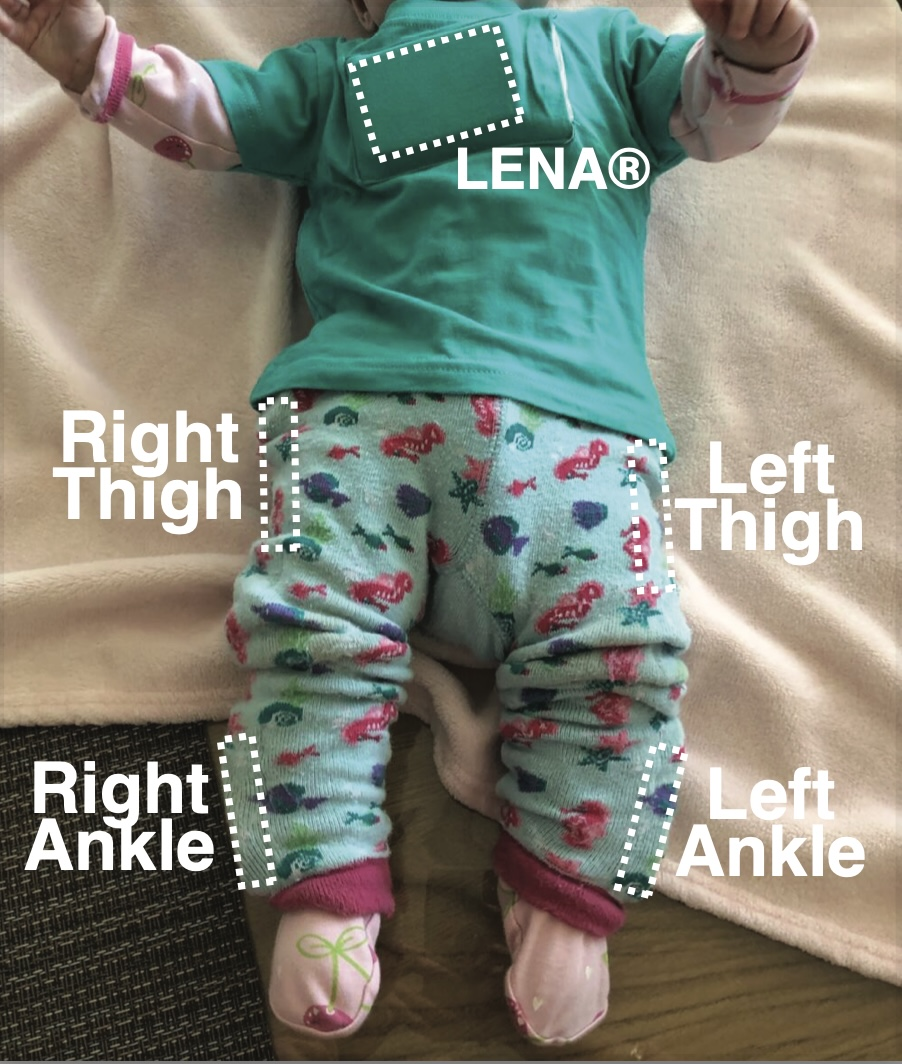
\includegraphics[width=0.75\linewidth]{figures/garment} 

}

\caption{Sensor garment worn by infant participant. Four IMUs were placed in interior pockets sewn into a tightly-fitting pair of infant leggings. White dashed rectangles mark the approximate locations of each sensor pocket (above the left and right ankles and on the left and right thighs, just below the thighs). A white dashed rectangle also marks the LENA audio recorder worn in a pocket on the infant's shirt.}\label{fig:garment}
\end{figure}

Videos were captured at 30 Hz using an action camera on a miniature tripod (Insta360 ONE R) that caregivers placed in the same room as the infant. Although recordings lasted 3 hours, they were divided into two video files of approximately 90 minutes temporally separated by a gap of 40-45 s. Caregivers received a log sheet to record times that infants napped and times that the sensor garment was removed from the infant (e.g., baths, diaper changes, errands).

\hypertarget{procedure}{%
\subsection{Procedure}\label{procedure}}

\begin{figure}

{\centering 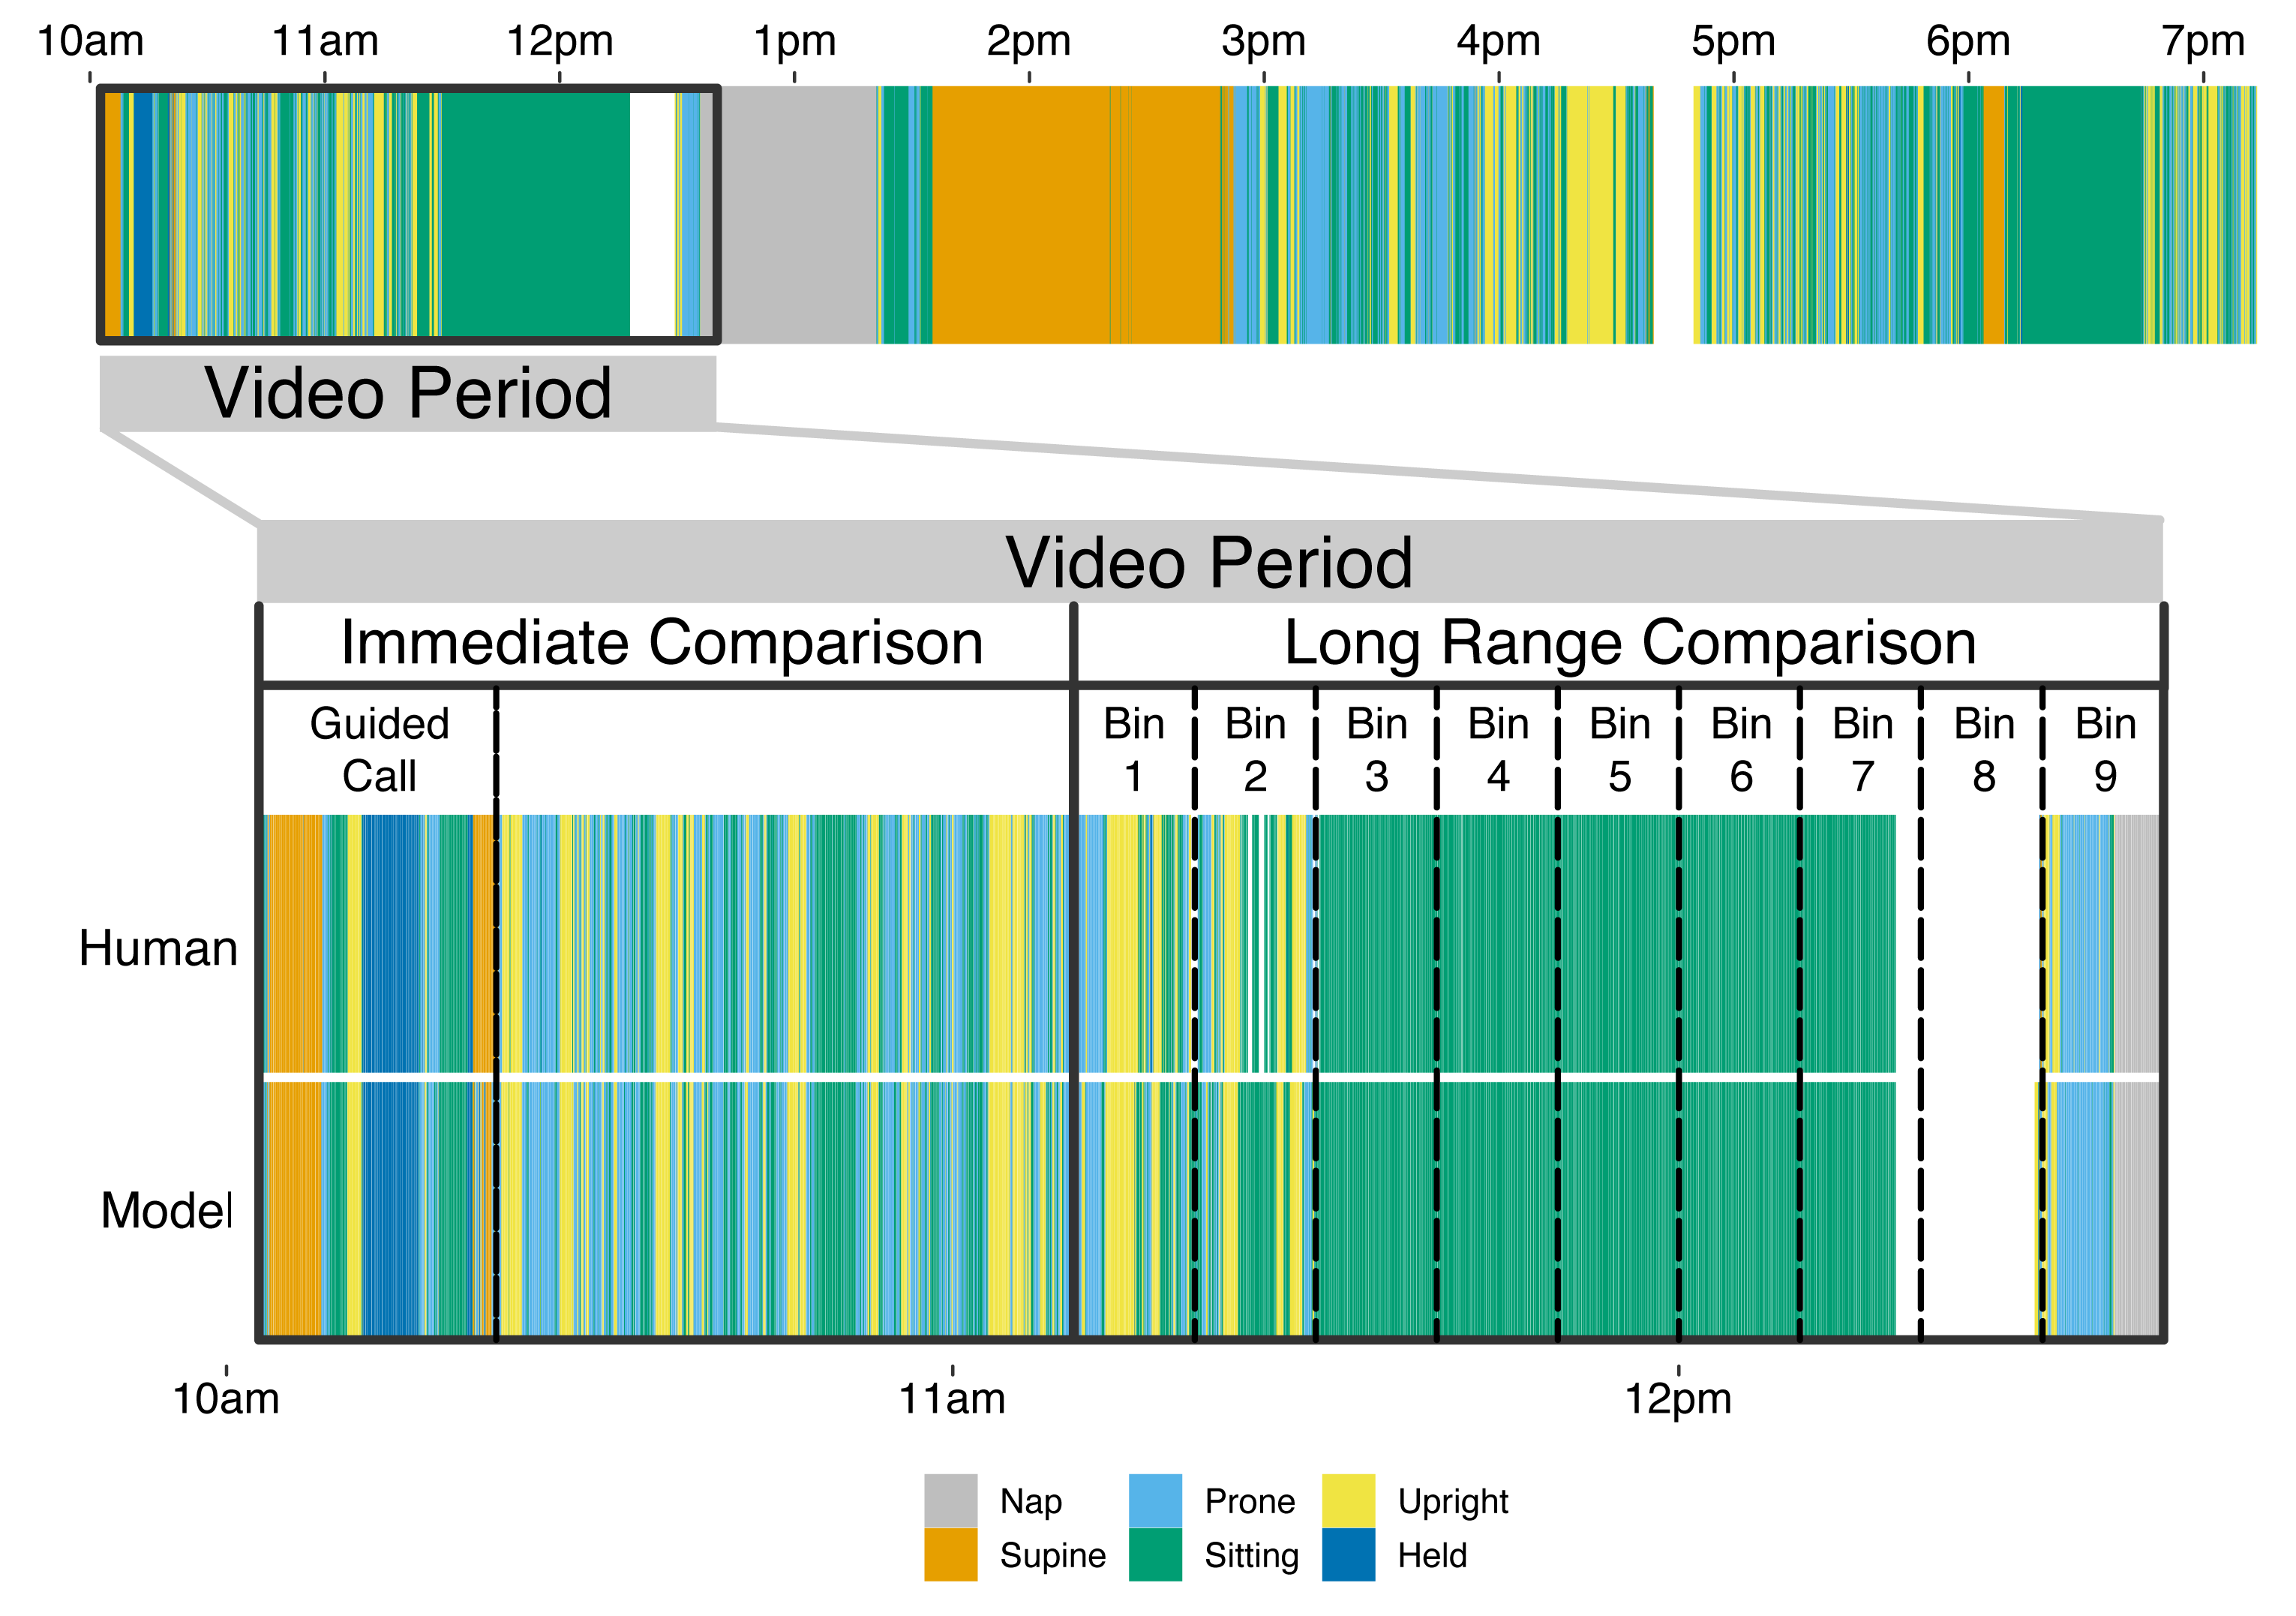
\includegraphics[width=0.99\linewidth]{figures/timeline} 

}

\caption{Timeline from an exemplar participant (older infant 15). The top row shows the model-predicted body position across the entire recording period. Annotations indicate when the video camera was turned on by the experimenter when arriving at the house, when the sensors were first placed on the infant, when the guided call took place, and when the video files were recorded. Gray areas on the timeline indicate naps, and white areas indicate times when the sensors were removed. The bottom row shows a zoomed-in view of the video period during which ground truth data were available. The top timeline shows human-coded body position and the bottom row shows model-predicted body position; these were the data used for validation. The first part of the video period was the proximal comparison, when video and motion data were highly synchronized. The second part of the video recording was the distal comparison that had coarser synchronization. Accuracy data for the distal comparison are provided overall and during 10-minute bins, marked by vertical dashed lines.}\label{fig:exemplar-timeline}
\end{figure}

Figure \ref{fig:exemplar-timeline} shows an exemplar timeline of the entire procedure and recording periods for a single participant. A researcher arrived at the participant's home in the morning and set each device to record while at the doorstep. To create a recognizable synchronization point between the video recording and IMU data, the researcher dropped the sensor garment containing the IMUs on a surface in view of the camera, as in \textcite{FranchakScott2021}. All the equipment---once recording and with synchronization information recorded---was placed inside a large bucket and left outside the family's front door. The researcher then called the caregiver on the phone and walked them through a set of procedures needed to properly set up the equipment and record video for ground truth human annotation of body position. At the start of this ``guided call'', the caregiver was instructed to place the camera in an area that captured the majority of the room. Next, they were asked to put the pair of leggings and shirt on their infant, with the researcher providing guidance about how to correctly orient the garments.

Afterwards, the researcher asked the caregiver to complete a number of guided activities with their infant. Within view of the camera, the caregiver was asked to place their infant in several different positions: lying supine, lying prone, sitting on the floor, standing upright, held by the caregiver while the caregiver walked back and forth, crawling, walking, and sitting in a restrained seat (e.g., high chair). Depending on the infants' age and motor skill level, the positions could be done independently or were completed with assistance from the caregiver. The researcher kept time to ensure at least 1 minute of behavior for each activity. Once completed, the caregiver was then instructed to play with their infant for 10 minutes within view of the camera to collect additional ground truth data.

Afterwards, they were asked to go about their day as usual with the infant wearing the sensor garment until their bedtime, only taking off the sensor for naps, baths, diaper changes, and trips out of the house. The caregiver logged the times the sensors were removed (blank areas in the timeline in Figure \ref{fig:exemplar-timeline}) or the child took a nap (gray areas in the timeline in Figure \ref{fig:exemplar-timeline}) so that those times could be excluded from analysis. The following day a researcher picked up the bucket of equipment.

Because the camera only had the battery life to record for \textasciitilde3 hours (automatically split into two 90-minute video files), this divided the day into different periods for analysis. As seen in the bottom of Figure \ref{fig:exemplar-timeline}), the \emph{video period} comprised the first three hours of recording starting from the researcher's arrival when they turned on the camera. The first 90-minute video file, termed the \emph{proximal comparison}, contained the activities during the guided call followed by a period during which infants and caregivers resumed their normal activities. Because this video contained the synchronization point, the data in this period had high temporal synchrony between IMU and video data. Synchronization errors were estimated to be less than 30-60 ms (1-2 video frames). The second video file comprised the \emph{distal comparison}. This video recorded the next 90 minutes of natural activity. However, because of a limitation in the camera, there was a variable gap of \textasciitilde40 s between the two videos, so synchronization in the distal comparison video was coarser, with estimated temporal offsets of \textasciitilde5 s in either direction.

\hypertarget{body-position-annotation}{%
\subsection{Body Position Annotation}\label{body-position-annotation}}

The proximal and distal comparison videos for each participant were annotated by trained human coders to identify infant \emph{body position} into one of 5 mutually-exclusive categories following the definitions in prior work \autocite{FranchakScott2021}: supine, prone, sitting, upright, or held by caregiver. All coding was done using Datavyu software (datavyu.org). A Databrary repository contains the entire video recording, coding files, and raw IMU data for a single participant (\url{https://nyu.databrary.org/volume/1580}).

Supine was coded when the infant was lying on their back, on their side, or was reclined up to a 45 Prone was coded when the infant was lying on their stomach, was stationary supported by the hands/knees or the hands/feet, or was crawling. We scored sitting to include any form of the following seated positions: 1) infants sat with their buttocks on a surface, such as on the floor or a caregiver's lap, 2) infant was in a kneeling-sit position, in which their knees were on the ground with their legs tucked underneath the buttocks, and 3) infant was in a seating device, such as a high chair, that kept the torso oriented perpendicular to the ground (a reclined position, such as in a young infant's car seat, would be counted as supine). Upright was coded when the infant was standing or squatting on the ground with two feet or walking (regardless of whether infants' balance was assisted by a caregiver or with their hands holding onto something for support). Our goal in creating a category for ``held by caregiver'' was to separate times when infants were in control of their body position from times when they were suspended in the air (rather than resting on furniture or a surface). Held was coded when infants were carried off of the groun. However, when the caregiver was sitting with the infant in their lap the infant's body position was coded as if the caregiver was a surface (e.g., if the infant was sitting on the caregiver's lap this was coded as sitting). Times during the video when the infant was out of view were excluded. Periods when the sensor garment was adjusted or taken off the infant were also excluded, as were transitions between body positions.

A primary coder completed annotation for the full length of the video, while an independent reliability coder completed annotation for the first thirty minutes of each video. Interrater reliability was based on the proportion of video frames that the two coders chose the same body position code. Overall agreement averaged 90.9\% across video files, ranging from 68.4\%-100\% for individual video files. Cohen's kappa averaged 86.1\% across video files, ranging from 31.0\%-100\% for individual video files.

\hypertarget{body-position-classification}{%
\subsection{Body Position Classification}\label{body-position-classification}}

The same machine learning classification process was used as in prior work \autocite{FranchakScott2021}. Using the synchronization point, human-coded body annotations from video were linked to the corresponding times in the IMU time series data. A single, merged dataset was created with synchronized accelerometer signals (in three orientations: X, Y, and Z) and gyroscope signals (in three orientations: roll, pitch, and yaw) for each of the four sensors (left thigh, right thigh, left ankle, right ankle) with the corresponding timestamp and body position code using the \emph{timetk} package \autocite{DanchoVaughan2023} and the \emph{lubridate} package \autocite{GrolemundWickham2011} in R version 4.1.2 \autocite{R42}.

Classification training and prediction was conducted on a windowed dataset that summarized the raw, 62.5 Hz motion signals within 4-s windows. Data were reduced in time by creating overlapping moving windows (4-s long, comprising 250 samples) starting each second, which is a common unit of analysis in prior studies of human activity classification \autocite{FranchakScott2021,NamPark2013,AiraksinenRasanen2020}. For each 4-s window, we aggregated the 250 samples to create single scores for a variety of motion features---summary statistics that could be fed into the machine learning model. The minimum, maximum, 25th percentile, 75th percentile, mean, median, skew, kurtosis, standard deviation, and sum were computed for each signal (e.g., right thigh X linear acceleration, left ankle pitch angular acceleration). The 10 summary statistics and 24 sensor signals generated 240 columns of motion features that described movement within each window. Furthermore, a series of cross-sensor and cross-orientation summaries (such as the correlation, magnitude, and difference between pairs of sensors) added an additional 196 columns of motion features. The 436 total motion features corresponded to a single body annotation code for each 4-s window. Windows were only used for training/testing if they contained a single body position for \textgreater{} 75\% (3 s) of time within the window to ensure that motion signals could be linked to an unambiguous example of each behavior.

The resulting windowed dataset was used for machine learning classification and validation. For each analysis reported in the results, a subset of data were defined as a ``training'' set and another, independent portion of the data were defined as a ``testing'' set (further described below). Random forest models \autocite{Breiman2001} used the training set to learn the body position label for each window from the set of 436 motion features using the \emph{randomForest} package \autocite{LiawWiener2002}. The resulting random forest model could later be applied to a set of testing data with the \emph{predict} function.

\hypertarget{data-sharing-and-transparency}{%
\subsection{Data Sharing and Transparency}\label{data-sharing-and-transparency}}

Three online repositories contain openly shared data, materials, and analysis code. A Databrary repository (\url{https://nyu.databrary.org/volume/1580}) includes an exemplar participant's recording session, with the raw video data files, the Datavyu annotations of those video files, a log file with machine-readable synchronization points and nap/diaper change times, and accelerometer and gyroscope data for each of the 4 sensors. A GitHub repository (\url{https://github.com/JohnFranchak/body_position_classification_example}) contains the exemplar participant's data and source code to: 1) synchronize IMU and video annotations, 2) calculate windowed motion features for their data, and 3) train and test the body position classifier using an ``individual model''. Because of the overall size of the full dataset and the computational power/time required to synchronize and create windowed datasets for each session, it would not be feasible to reproduce the calculations for all 34 sessions. However, in a second Github repository (\url{https://github.com/JohnFranchak/body_position_classification_ms}) we share the full results of those computations: The dataset of windowed motion features with corresponding body position codes used to validate the method. This reproducible manuscript created in RMarkdown and \emph{papaja} \autocite{papaja} can be regenerated from those data files for full computational transparency.

\hypertarget{results}{%
\section{Results}\label{results}}

We report three sets of results based on 34 full-day testing sessions resulting in a total of 302 hours of movement recording.

\hypertarget{assess-the-proximal-accuracy-of-body-position-classification-models}{%
\subsection{Assess the Proximal Accuracy of Body Position Classification Models}\label{assess-the-proximal-accuracy-of-body-position-classification-models}}

\begin{figure}

{\centering 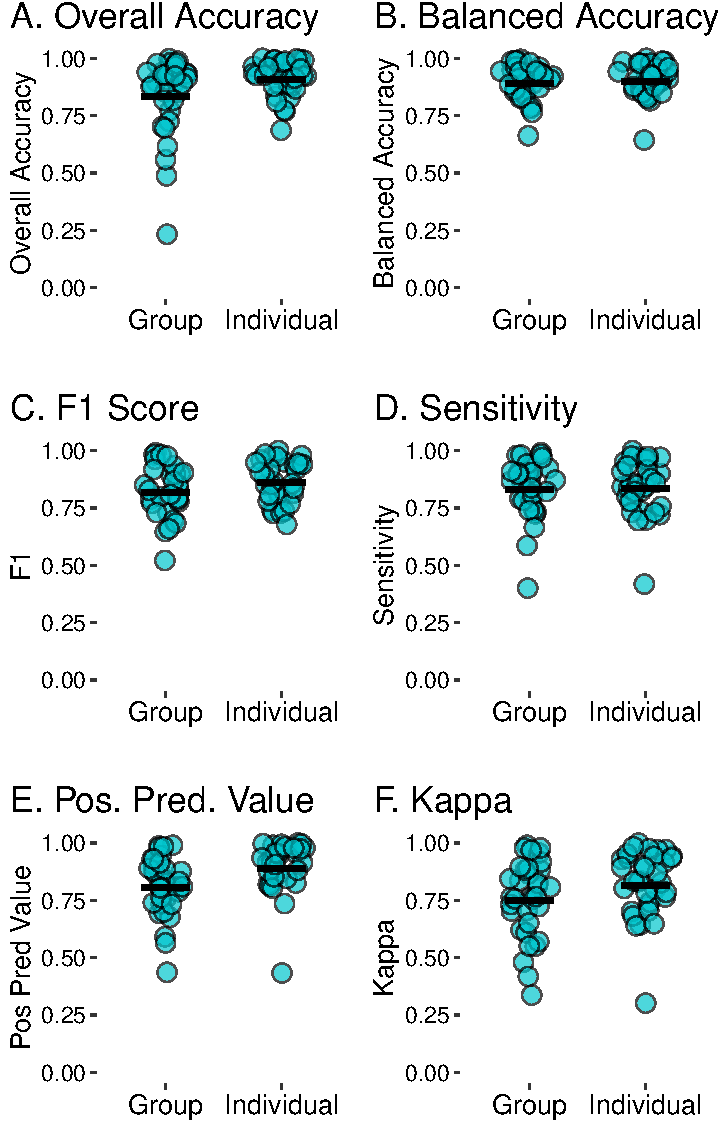
\includegraphics{manuscript_files/figure-latex/metrics-1} 

}

\caption{Metrics of agreement between human-annotated body position and model predictions of body position from the proximal comparison period. Overall accuracy (A) and Cohen's Kappa (B) are plotted separately for group models and individual models. Each blue circle represents that accuracy for each recording session. Horizontal black bars indicate the mean across sessions.}\label{fig:metrics}
\end{figure}

\begin{table}[tbp]

\begin{center}
\begin{threeparttable}

\caption{\label{tab:metrics-table}Model performance metrics (overall accuracy, Cohen's Kappa, sensitivity, positive predictive value) from the proximal comparison period. Descriptive statistics are shown separately for group and individual models.}

\begin{tabular}{lllllll}
\toprule
 & \multicolumn{3}{c}{Group} & \multicolumn{3}{c}{Individual} \\
\cmidrule(r){2-4} \cmidrule(r){5-7}
Metric & Median & Mean & SD & Median & Mean & SD\\
\midrule
Overall Accuracy & 0.894 & 0.846 & 0.131 & 0.933 & 0.916 & 0.072\\
Kappa & 0.768 & 0.746 & 0.161 & 0.849 & 0.821 & 0.143\\
Sensitivity & 0.856 & 0.825 & 0.127 & 0.847 & 0.841 & 0.119\\
Pos Pred Value & 0.826 & 0.810 & 0.125 & 0.928 & 0.899 & 0.107\\
\bottomrule
\end{tabular}

\end{threeparttable}
\end{center}

\end{table}

\renewcommand{\arraystretch}{.75}

\begin{table}[tbp]

\begin{center}
\begin{threeparttable}

\caption{\label{tab:metrics-by-class}Model performance metrics for each body position (supine, prone, sitting, upright, and held) during the proximal comparison period, shown separately for group and individual models.}

\begin{tabular}{llllllll}
\toprule
 &  & \multicolumn{3}{c}{Group} & \multicolumn{3}{c}{Individual} \\
\cmidrule(r){3-5} \cmidrule(r){6-8}
Metric & Position & Median & Mean & SD & Median & Mean & SD\\
\midrule
Kappa & Supine & 0.907 & 0.764 & 0.295 & 0.983 & 0.912 & 0.166\\
 & Prone & 0.968 & 0.860 & 0.259 & 0.942 & 0.841 & 0.246\\
 & Sitting & 0.816 & 0.702 & 0.297 & 0.915 & 0.887 & 0.127\\
 & Upright & 0.707 & 0.673 & 0.281 & 0.822 & 0.741 & 0.236\\
 & Held & 0.732 & 0.726 & 0.209 & 0.826 & 0.727 & 0.277\\ \midrule
Sensitivity & Supine & 1.000 & 0.905 & 0.180 & 1.000 & 0.954 & 0.129\\
 & Prone & 1.000 & 0.894 & 0.234 & 0.974 & 0.849 & 0.272\\
 & Sitting & 0.910 & 0.811 & 0.257 & 0.964 & 0.915 & 0.136\\
 & Upright & 0.837 & 0.730 & 0.297 & 0.891 & 0.786 & 0.253\\
 & Held & 0.852 & 0.772 & 0.228 & 0.773 & 0.702 & 0.312\\ \midrule
Pos Pred Value & Supine & 0.995 & 0.828 & 0.292 & 1.000 & 0.932 & 0.134\\
 & Prone & 0.987 & 0.877 & 0.236 & 1.000 & 0.892 & 0.210\\
 & Sitting & 0.896 & 0.802 & 0.261 & 0.972 & 0.945 & 0.079\\
 & Upright & 0.839 & 0.739 & 0.283 & 0.923 & 0.825 & 0.228\\
 & Held & 0.852 & 0.794 & 0.240 & 0.943 & 0.899 & 0.134\\
\bottomrule
\end{tabular}

\end{threeparttable}
\end{center}

\end{table}

The first set of analyses use data from the proximal comparison to determine the ``best case'' accuracy of the models, training and testing on similar types of data. The high degree of temporal synchronization between video and motion data during this period makes it possible to link human-coded body position annotations to each 4-s window of motion data, providing ground truth data for model training and testing. As in past work \autocite{FranchakScott2021}, we compared two types of models: \emph{group models} and \emph{individual models}. To assess the accuracy of body position classification for each recording session, we reserved the (temporally) last 25\% of a session's proximal comparison data as the testing set. The testing set was never used as training data. The two types of models differed based on what data were used during training: A group model was trained for each session using an aggregated dataset containing the first 75\% of all \textbf{other} sessions' proximal comparison data. This leave-one-out cross-validation tested the generalization of the model to a recording session that was not used at all in the training set. In contrast, individual models were trained using the first 75\% of a recording session, then tested against the (temporally) last 25\% of the same session. The individual model tests whether earlier training data generalize to later testing data within an individual participant's recording. In both cases, the testing set was the same, allowing for direct comparison between the two modeling approaches. Figure \ref{fig:metrics}, Table \ref{tab:metrics-table}, and Table \ref{tab:metrics-by-class} summarize the performance of group and individual models using standard metrics for classification.

\begin{table}[tbp]

\begin{center}
\begin{threeparttable}

\caption{\label{tab:metrics-reduce}Median, mean, and SD of overall accuracy calculated with different sets of sensor features. The top row shows performance using all features calculated from the four sensors. Rows 2-5 show accuracy using pairs of sensors (left thigh and ankle, right thigh and ankle, left and right thigh, left and right ankle), and rows 6-9 show accuracy using each individual sensor.}

\begin{tabular}{lllllll}
\toprule
 & \multicolumn{3}{c}{Group} & \multicolumn{3}{c}{Individual} \\
\cmidrule(r){2-4} \cmidrule(r){5-7}
Sensors & Median & Mean & SD & Median & Mean & SD\\
\midrule
All & 0.894 & 0.846 & 0.131 & 0.933 & 0.916 & 0.072\\ \midrule
Left Hip/Ankle & 0.891 & 0.824 & 0.177 & 0.915 & 0.901 & 0.071\\
Right Thigh/Ankle & 0.842 & 0.800 & 0.167 & 0.897 & 0.898 & 0.086\\
Both Thighs & 0.859 & 0.791 & 0.195 & 0.907 & 0.898 & 0.072\\
Both Ankles & 0.797 & 0.719 & 0.196 & 0.864 & 0.844 & 0.108\\ \midrule
Left Thigh & 0.842 & 0.762 & 0.208 & 0.889 & 0.872 & 0.077\\
Left Ankle & 0.717 & 0.667 & 0.208 & 0.851 & 0.825 & 0.117\\
Right Thigh & 0.846 & 0.772 & 0.178 & 0.896 & 0.876 & 0.092\\
Right Ankle & 0.704 & 0.683 & 0.160 & 0.830 & 0.819 & 0.114\\
\bottomrule
\end{tabular}

\end{threeparttable}
\end{center}

\end{table}

\hypertarget{overall-accuracy}{%
\subsubsection{Overall Accuracy}\label{overall-accuracy}}

Overall accuracy (Figure \ref{fig:metrics}A) represents the proportion of 4-s windows in the testing set in which the model prediction matched the human annotation of body position. Overall accuracy for group models (\emph{M} = 0.85) was slightly lower than accuracy for individual models (\emph{M} = 0.92). Although overall accuracy from our semi-supervised, in-home data collection did not match the near-perfect accuracy (.95-.98) found in prior in-lab studies \autocite{FranchakScott2021,AiraksinenRasanen2020}, both models approached the level of agreement found between two human coders (\emph{M} = .906). Most likely, lower accuracy in the current study results from the more variable and complex behavior observed in a a semi-supervised setting rather than from a difference in the quality of the classification model; although the first part of the proximal period was guided by the experimenter during a brief phone call, the remainder of the proximal period included natural behavior. Visual inspection of Figure \ref{fig:metrics}A shows that accuracy values were heavily skewed, with many approaching perfect accuracy but a few sessions with very poor accuracy. Looking at the median performance suggests that the difference between models was not considerable for the typical participant (group median accuracy = 0.89; individual median accuracy = 0.93).

As in \textcite{AiraksinenRasanen2020}, overall accuracy decreased when fewer sensors were used. Table \ref{tab:metrics-reduce} compared overall accuracy for all four sensors (top row), pairs of 2 sensors (rows 2-5), and single sensors (rows 6-9). The highest accuracy was observed when using all four sensors (group model \emph{M} = 0.846; individual model \emph{M} = 0.916), and the lowest when using only a single sensor (left ankle group model \emph{M} = 0.667; right ankle individual model \emph{M} = 0.819). Accuracy for some pairs approached 4-sensor accuracy: Left ankle and thigh had group model accuracy of \emph{M} = NA and individual model accuracy of \emph{M} = NA, only 2.2\% and 1.5\% worse than using all four sensors. Other pairings were less accurate; notably, using both ankles resulted in group model accuracy of \emph{M} = 0.719 and individual model accuracy of \emph{M} = 0.844, 12.7\% and 7.2\% worse than using all four sensors.

\hypertarget{cohens-kappa}{%
\subsubsection{Cohen's Kappa}\label{cohens-kappa}}

Strong overall accuracy can be misleading when the relative frequency of different classes is unbalanced. Accordingly, we report Cohen's kappa, a commonly-used metric that penalizes missing rare events (Figure \ref{fig:metrics}B), and we provide classification metrics for each individual body position (Table \ref{tab:metrics-by-class}) to account for imbalance in body position rates within and between individuals. Similar to overall accuracy, kappa values were strong for both model types with group kappas (\emph{M} = 0.75) somewhat worse compared with individual kappas (\emph{M} = 0.82). Guidelines for interpreting kappa statistics \autocite{LandisKoch1977} consider 0.81--1.00 ``Almost Perfect,'' 0.61--0.80 ``Substantial,'' 0.41--0.60 ``Moderate,'' 0.21-- 0.40 ``Fair,'' and 0--0.20 ``Slight to Poor'', indicating that agreement for most group and individual model predictions fell in the Substantial to Almost Perfect range.

As in past work \autocite{FranchakScott2021,AiraksinenRasanen2020}, all body positions were accurately classified even though performance varied somewhat between positions. As Table \ref{tab:metrics-by-class} shows, mean kappa statistics were strongest for prone (group \emph{M} = 0.860, individual \emph{M} = 0.841) and supine (group \emph{M} = 0.764, individual \emph{M} = 0.912). Sitting performance fell in the middle, and was considerably worse for group models than individual models (group \emph{M} = 0.702, individual \emph{M} = 0.887). Held (group \emph{M} = 0.726, individual \emph{M} = 0.727) and upright (group \emph{M} = 0.673, individual \emph{M} = 0.741) performance was the least accurate, however, average performance was still within the ``Substantial'' range.

\hypertarget{sensitivity-and-positive-predictive-value}{%
\subsubsection{Sensitivity and Positive Predictive Value}\label{sensitivity-and-positive-predictive-value}}

Sensitivity refers to the proportion of events of a given position that were correctly identified (e.g., out of 100 human-coded sitting windows, how many of those windows did the model correctly classify as sitting?). High sensitivity means that events are unlikely to be missed. In contrast, positive predictive value (PPV) refers to the proportion of events classified for a given position that actually belonged to that position (e.g., if the model said a baby was upright during 100 windows, how many of those windows were indeed human-coded upright events?). High PPV means that we can be confident in the event label. Table \ref{tab:metrics-by-class} shows the sensitivity and PPV by body position class for group and individual models. For group models, sensitivity and PPV were similar: They were highest for supine, prone, and sitting (the most accurately identified class) and lowest for upright and held. Results for individual models were similar to group models, with the exception of a somewhat lower sensitivity score for held. Overall, the results suggest a reasonable balance between sensitivity and PPV among different body position classes for both model types.

\hypertarget{measure-the-distal-accuracy-of-body-position-classification-models}{%
\subsection{Measure the Distal Accuracy of Body Position Classification Models}\label{measure-the-distal-accuracy-of-body-position-classification-models}}

\begin{figure}

{\centering 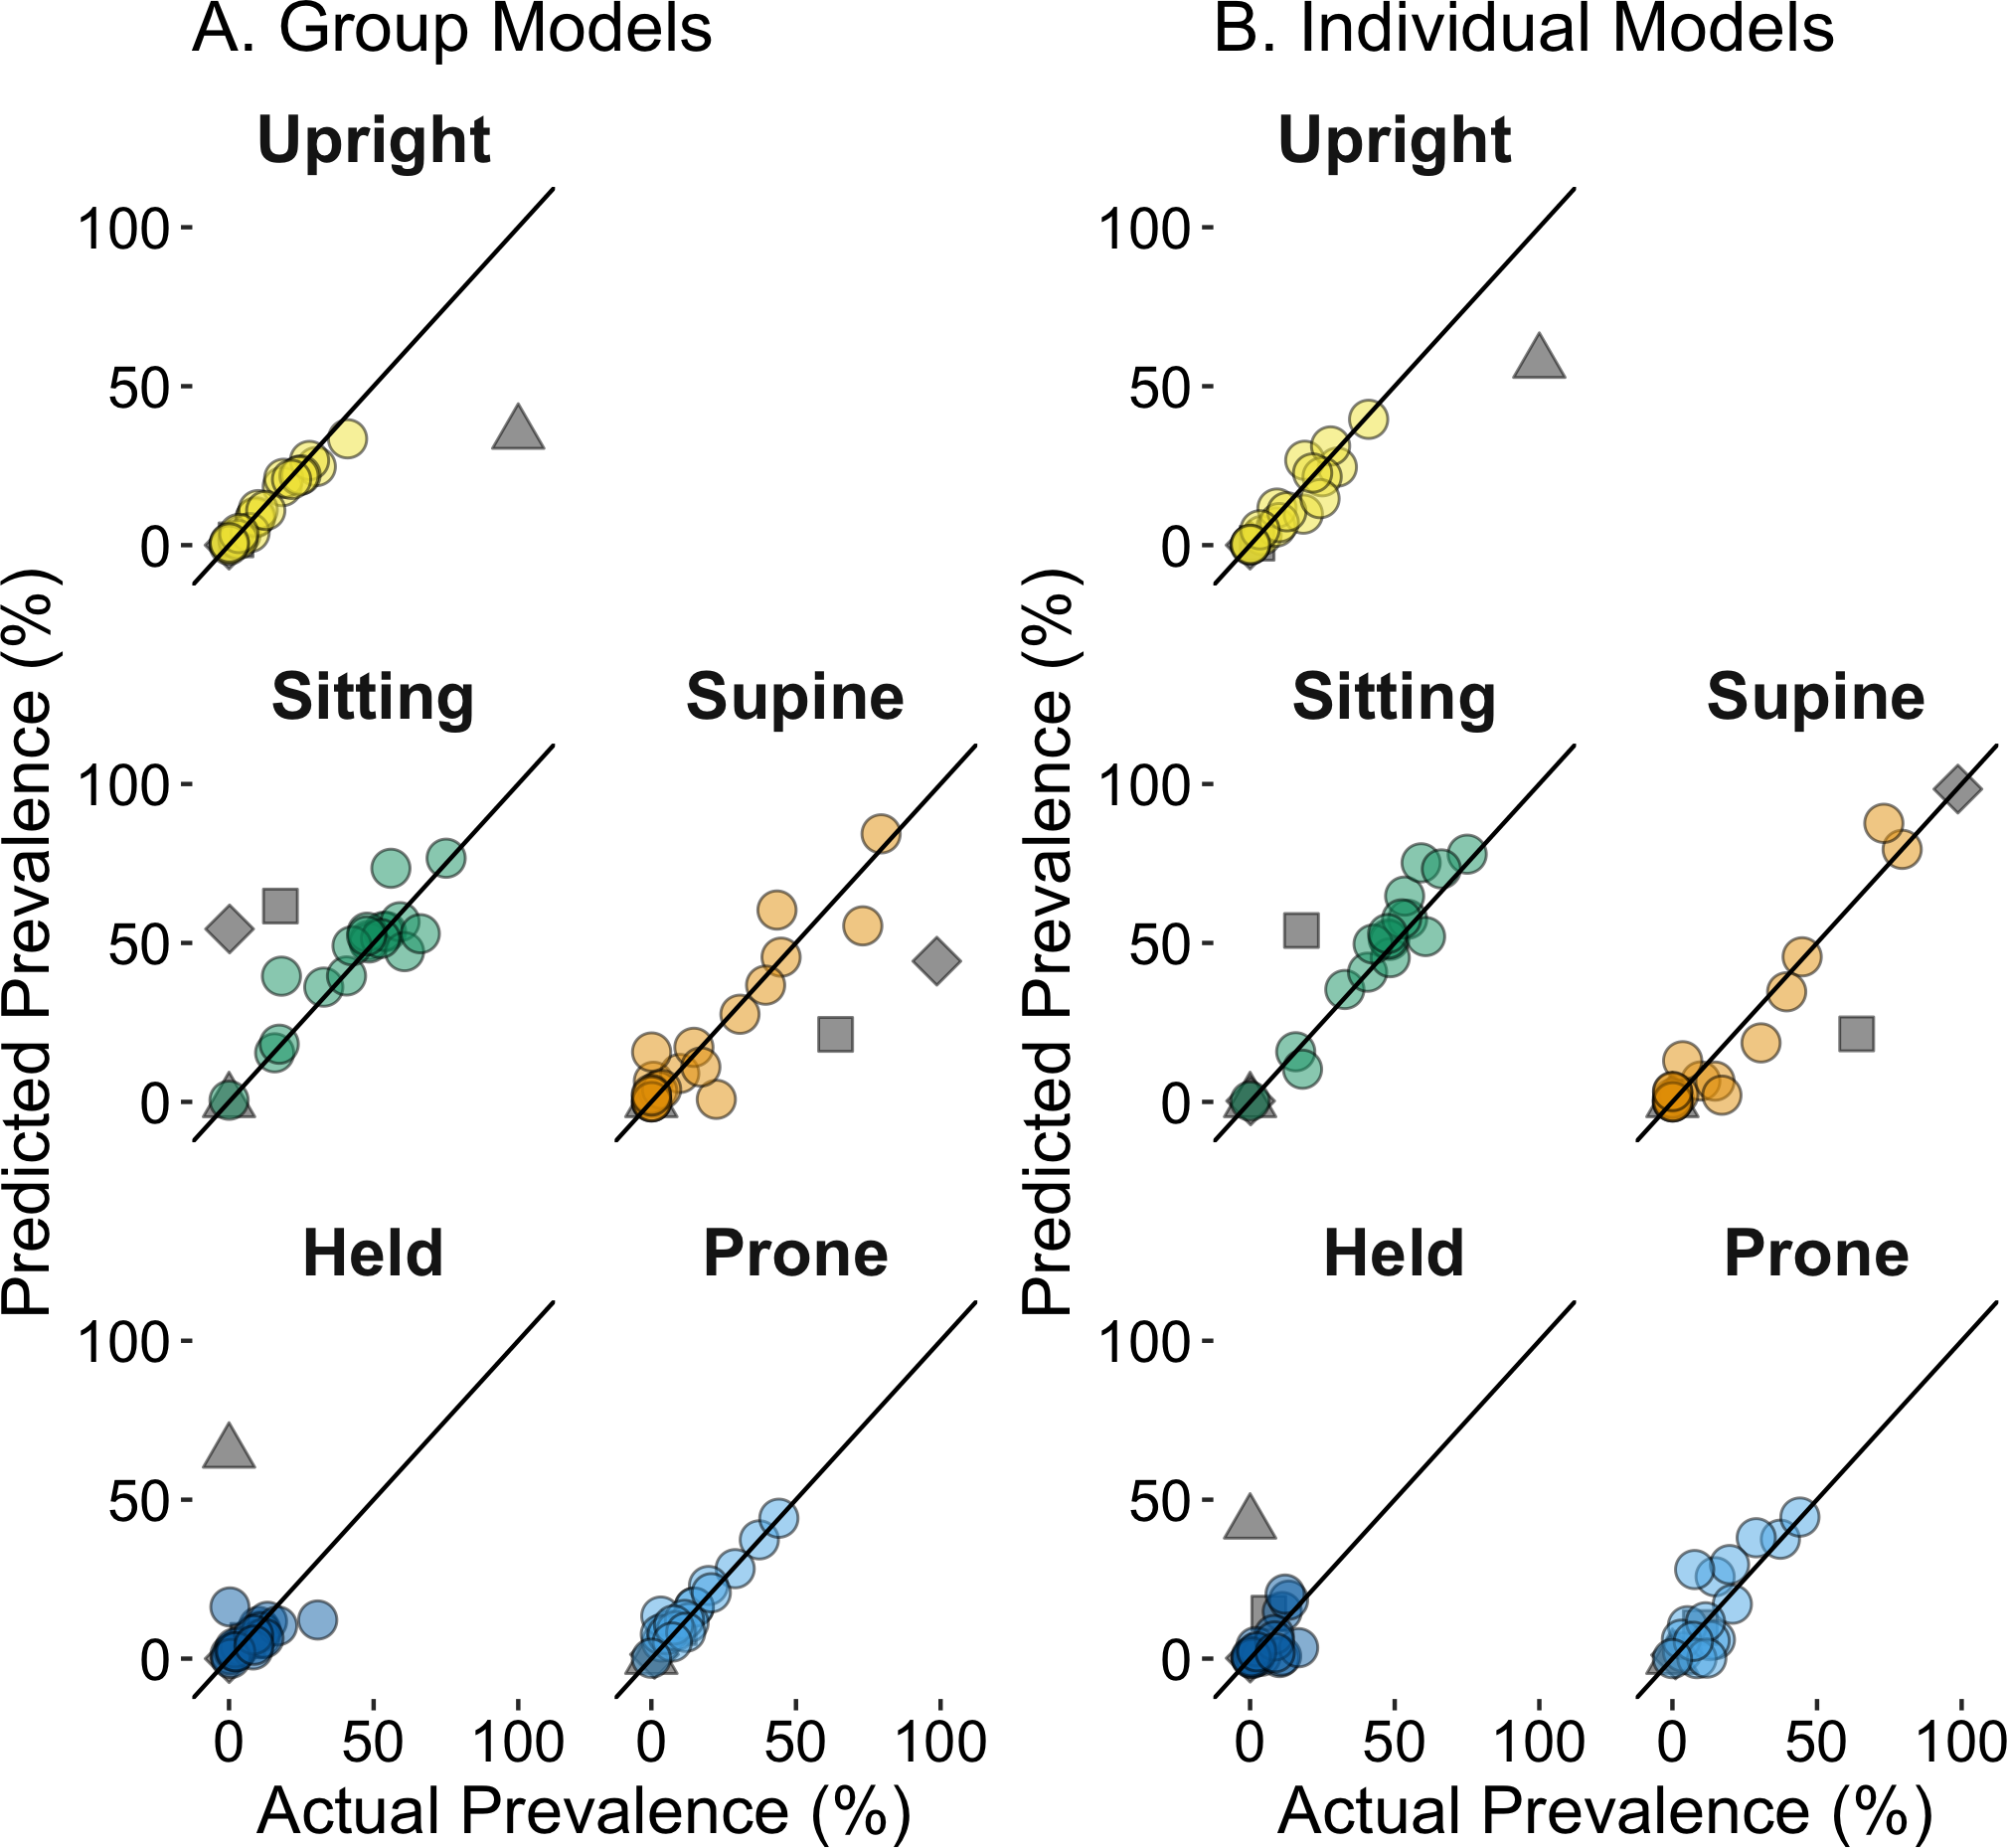
\includegraphics{manuscript_files/figure-latex/part2overall-1} 

}

\caption{Overall agreement between human-coded body position and model-predicted body position in the distal comparison. Agreement for group models is shown in (A) and agreement for individual models is shown in (B). Plots are shown separately for each body position with a reference line that indicates perfect agreement; each point in a plot represents data for a single session. The two outlier participants are plotted in dark gray, with a different shape marking each individual. }\label{fig:part2overall}
\end{figure}

\begin{table}[tbp]

\begin{center}
\begin{threeparttable}

\caption{\label{tab:pt2overalltable}Correlations between human-coded and model-predicted body position durations across the entire distal comparison period. Correlations are provided within each body position and overall. Correlations are presented separately for group and individual models with and without the two outlier participants.}

\begin{tabular}{lllll}
\toprule
 & \multicolumn{2}{c}{With Outliers} & \multicolumn{2}{c}{Without Outliers} \\
\cmidrule(r){2-3} \cmidrule(r){4-5}
Position & Group & Individual & Group & Individual\\
\midrule
Supine & 0.88 & 0.98 & 0.94 & 0.97\\
Prone & 0.97 & 0.86 & 0.97 & 0.84\\
Sitting & 0.79 & 0.97 & 0.91 & 0.95\\
Upright & 0.63 & 0.83 & 0.99 & 0.95\\
Held & 0.02 & 0.04 & 0.73 & 0.60\\ \midrule
Overall & 0.80 & 0.91 & 0.95 & 0.96\\
\bottomrule
\end{tabular}

\end{threeparttable}
\end{center}

\end{table}

The first set of results showed that group and individual models trained from data during the proximal comparison period were within the proximal period. In the next analysis, we examine long-term performance by testing how accurately models trained from the proximal period could predict body position during the distal comparison period. A single group model was created using all sessions' proximal period training data (rather than group models leaving out a single session); the same individual models were used. Distal videos had only coarse temporal synchrony with motion recordings which precluded calculating accuracy based on the proportion of matching events. Instead, we summed the amount of time infants were predicted to be in each of the 5 body position categories from the model and compared that to the summed time for the body positions based on human coding \autocite{YaoPlotz2019,FranchakScott2021}.

Whereas the proximal analyses used all 34 sessions, this was not possible in the distal comparison. Because the start of the visit was scheduled during a time when the infant was awake, it was common for a nap to follow the proximal period. Nine sessions were excluded because the infant was either napping or otherwise not on camera during the entire 90-minute distal recording. Three additional sessions were excluded because a caregiver accidentally turned off the video camera (\emph{n} = 1) or (purposefully) left the house (\emph{n} = 2). This left 22 sessions with usable distal comparison data.

\hypertarget{overall-agreement-during-the-distal-comparison}{%
\subsubsection{Overall Agreement During the Distal Comparison}\label{overall-agreement-during-the-distal-comparison}}

Figure \ref{fig:part2overall} and Table \ref{tab:pt2overalltable} summarize the overall agreement during the distal comparison period. For each session, we calculated the actual time spent in each body position (out of times the infant was visible on camera and awake) using human annotated body position (x-axis on Figure \ref{fig:part2overall}). Predicted time was calculated the same way for group and individual model predictions, omitting the off-camera and nap periods to make a direct comparison. Overall---across participants and across body position classes---agreement was strong: The correlation between group model predictions and human-coded time was \emph{r} = 0.80, and the correlation between individual model predictions and human-coded time was \emph{r} = 0.91. As in the proximal comparison, agreement varied somewhat between body positions; in particular, agreement for held was poor. Unlike in the proximal period, some body positions were better predicted by group models and others by individual models.

Visual inspection of Figure \ref{fig:part2overall} indicated two extreme outliers, which we marked by a gray square and a gray diamond. The ``gray square'' outlier had significant confusion between sitting and supine classification. Reviewing the video indicated that this participant spent a long period of time in a seating device that was reclined almost exactly at 45 degrees, making it difficult to determine if the infant was sitting or supine. The infant also spent a long time in the mother's arms in an ambiguous supine/sitting position. This participant's proximal accuracy was also poor because similar ambiguities appeared during the initial recording. In contrast, the ``gray diamond'' outlier had strong proximal accuracy, with confusion only arising in the distal period between upright and held categories. Reviewing the video showed that all disagreements occurred when the infant was in a baby walker; human coders scored this as ``upright'' but the models predicted it as ``held''. Most likely, the infant's movements in the baby walker were more similar to how a baby moved while carried, and unlike how most infants moved while walking upright.

What is notable about both outliers is that disagreements were restricted to a particular border case (supine vs.~sitting; upright vs.~held); accuracy for other classes remained strong. This suggests that their poor performance came as a result of spending a long time in an ambiguous position, not the result of the entire model failing to generalize to the later time period (or an error in sensor placement, such as if the parent removed the leggings and put them on backwards after a diaper change). To better capture the typical level of agreement, we report all correlations in Table \ref{tab:pt2overalltable} excluding the two outliers. Overall agreement among the non-outlier sessions was excellent for both group models (\emph{r} = 0.95) and individual models (\emph{r} = 0.96).

\begin{figure}

{\centering 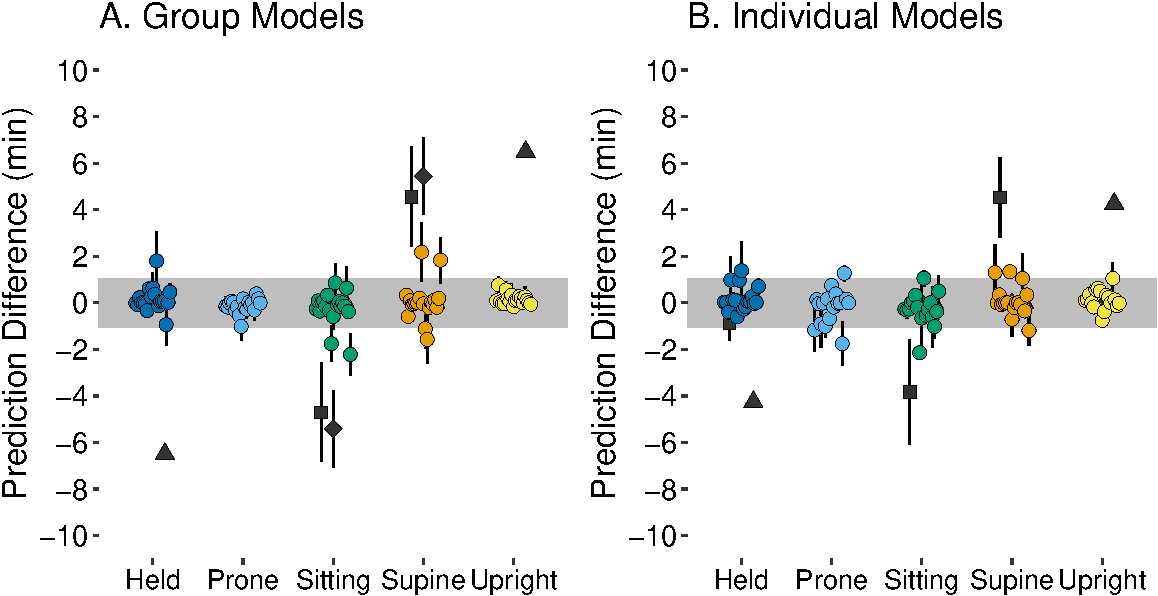
\includegraphics{manuscript_files/figure-latex/part2bins-1} 

}

\caption{Prediction difference (difference in minutes between human-coded and model-predicted body position) for 10-minute bins in the distal comparison period. Each point shows the mean and SE for a single recording session for each body position, summarizing the prediction difference for each of their 10-minute bins. Points falling within the gray shaded region indicate that average prediction errors were less than 1 minute. Performance is plotted separately for (A) group models and (B) individual models. The two outlier participants are plotted in dark gray, with a different shape marking each individual.}\label{fig:part2bins}
\end{figure}

\begin{table}[tbp]

\begin{center}
\begin{threeparttable}

\caption{\label{tab:pt2binstable}Correlations between human-coded and model-predicted body position durations using 10-minute bins during the distal comparison period. Correlations are provided within each posture and overall, and computed separately using group and individual models with and without outlier participants.}

\begin{tabular}{lllll}
\toprule
 & \multicolumn{2}{c}{With Outliers} & \multicolumn{2}{c}{Without Outliers} \\
\cmidrule(r){2-3} \cmidrule(r){4-5}
Position & Group & Individual & Group & Individual\\
\midrule
Supine & 0.76 & 0.96 & 0.88 & 0.93\\
Prone & 0.96 & 0.90 & 0.96 & 0.89\\
Sitting & 0.72 & 0.93 & 0.89 & 0.92\\
Upright & 0.91 & 0.93 & 0.98 & 0.96\\
Held & 0.51 & 0.46 & 0.67 & 0.63\\ \midrule
Overall & 0.80 & 0.94 & 0.92 & 0.94\\
\bottomrule
\end{tabular}

\end{threeparttable}
\end{center}

\end{table}

\hypertarget{short-timescale-agreement-during-the-distal-comparison}{%
\subsubsection{Short-Timescale Agreement during the Distal Comparison}\label{short-timescale-agreement-during-the-distal-comparison}}

Although overall aggregate agreement in the distal comparison was strong, it is important to show that similarly strong agreement is found within a shorter timescale. We repeated the agreement analysis after dividing the distal comparison period into nine 10-minute bins (marked by vertical dashed lines in Figure \ref{fig:exemplar-timeline}). Infants had varying numbers of 10-minute bins depending on how much time they were awake and on camera. Bins were included only if there was \textgreater{} 7 minutes of usable data. Table \ref{tab:pt2binstable} shows the agreement correlation coefficients for group and individual models, including and excluding the two outliers identified in the previous section. Performance at a short timescale was similar to performance overall: Overall agreement after excluding outliers was excellent for both group (\emph{r} = 0.92) and individual models (\emph{r} = 0.94). Within-position correlations were weakest for held and strongest for upright regardless of the model type. Agreement for prone was better for group models, whereas sitting and supine were better predicted by individual models.

To describe the observed amount of prediction error in 10-minute bins, we subtracted the predicted duration (in minutes) for each body position in each bin from the human coded duration in that bin to create a prediction difference score. A score of 0 would indicate no error; positive differences indicate that the model overestimated the amount of time in a position, whereas negative differences indicate underestimation. Figure \ref{fig:part2bins} plots the mean prediction difference for each session for each body position. The gray shaded area marks ± 1 minute of prediction error. Most session-averaged predictions fall within 1 minute of error without a clear bias towards overestimation or underestimation. For group models, we calculated the percentage of 10-min bins across participants that had errors \textless{} 1 minute: 94.62\% for held, 80.65\% for supine, 94.62\% for prone, 77.42\% for sitting, and 94.62\% for upright. For individual models, the percent of 10-min bins with \textless{} 1 minute of error was: 92.86\% for held, 88.10\% for supine, 88.10\% for prone, 83.33\% for sitting, and 96.43\% for upright.

\hypertarget{examine-the-data-quality-of-full-day-home-recordings}{%
\subsection{Examine the Data Quality of Full-Day Home Recordings}\label{examine-the-data-quality-of-full-day-home-recordings}}

\begin{figure}

{\centering 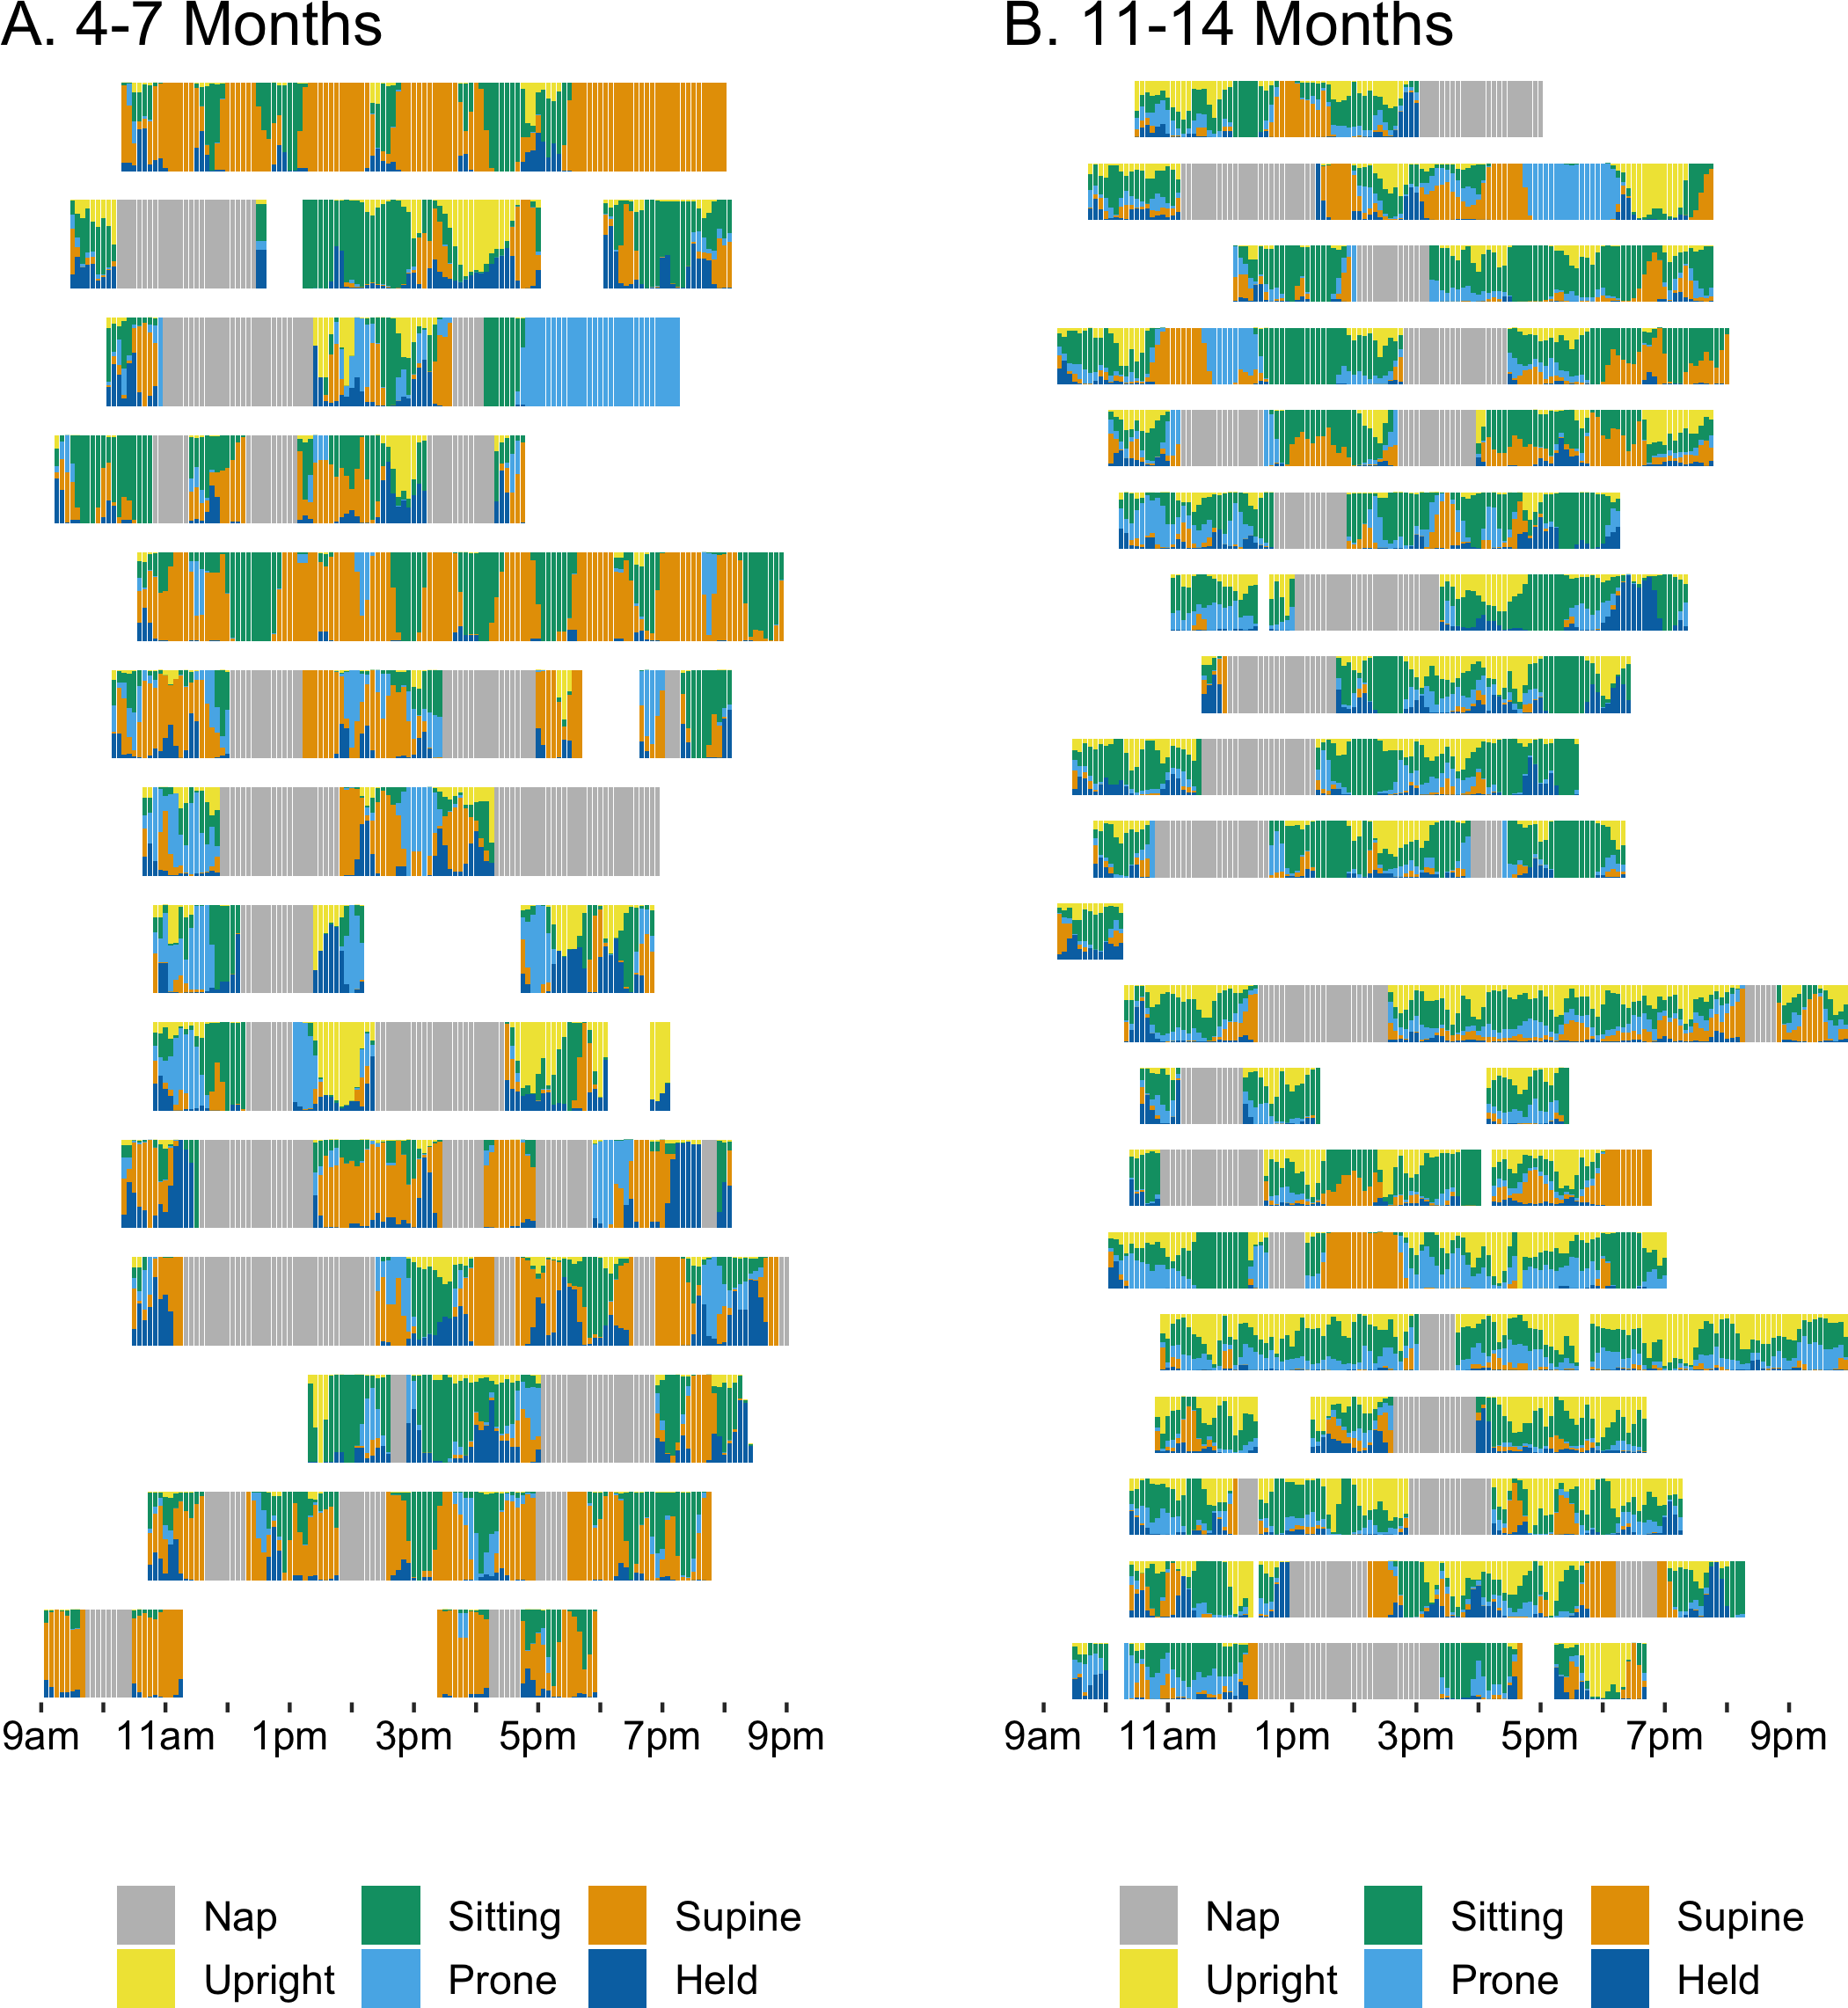
\includegraphics{manuscript_files/figure-latex/timelines-1} 

}

\caption{Full-day timelines for each individual recording session, split by (A) younger infants and (B) older infants. Each participant's timeline shows a stacked bar graph with the proportion of time spent in each of the body positions for every 5-minute period throughout the day, based on group model predictions of body position. The x-axis shows time of day. Caregiver-reported naps are marked by gray bars; blank gaps indicate caregiver-reported times that the sensor garment was removed for diaper changes, baths, or trips out of the house.}\label{fig:timelines}
\end{figure}

After the distal comparison video ended, caregivers were instructed to keep the sensors on their infants for the remainder of the day until infants went to bed, removing the sensors for naps, diaper changes, and trips out of the house. The algorithm was not designed to classify behavior during transportation (e.g., strollers, automobiles) so data collection was restricted to in-home behavior. The first two sets of results show that accuracy was consistently high across the proximal and distal recordings, providing confidence that predictions over the remainder of the day would continue to be accurate after the video recordings stopped. This leads to two final questions---how successfully did recordings capture infants' entire day, and how well do findings from full-day classification converge with findings that use other methodologies?

\hypertarget{how-well-did-recordings-capture-infants-entire-day}{%
\subsubsection{How Well Did Recordings Capture Infants' Entire Day?}\label{how-well-did-recordings-capture-infants-entire-day}}

Figure \ref{fig:timelines} depicts body position timelines across the day for each session, divided into younger (A) and older infants (B). Predictions from the group model were used to ensure that motion data were classified consistently across all sessions. Moreover, for infants who did not display all 5 body positions in the training period, group models were necessary to predict those behaviors across the entire day. Session start times ranged from 09:15 to 13:20 with a median of 10:25. Sometimes infants were unexpectedly asleep at the scheduled time, leading to a few sessions in which infants began wearing the sensors later than intended (such as \#11 in the younger group). With two exceptions, recordings lasted until the infants' bedtime. Older participant \#1 had the equipment picked up on the same day rather than the next day, so the recording ended at 17:00. Older participant \#11 wore the equipment in the morning, but the family left the house at 10:15 and remained out for the rest of the day, choosing not to put the equipment back on when they returned home in the late afternoon. Among those participants who wore the equipment until bedtime, recordings ended between 17:25 and 22:15 with a median of 19:20.

Among participants who wore the sensors from morning to bedtime, all infants wore the sensor garment during 100\% of the intended recording period, excluding the times caregivers were asked to remove the garment (naps, diaper changes, trips out of the house), based on caregiver logs of wear time. No caregiver reporting removing the garment for any other reason (such as infant discomfort), meaning that the majority of the time during the day either resulted in usable body position data or was excluded due to caregiver-reported naps (gray periods in Figure \ref{fig:timelines}). The total length of the recording period ranged from 6.92-11.75 hours with a median of 9.04 hours. Nap times reported during the recording period ranged from 0.00-4.99 hours with a median of 2.25 hours. Body position data were available to describe 37.3-100.0\% of the awake portion of the recording period (median = 100.0\%). Younger infant \#14 had the least portion of the waking day accounted for; the family left the house to run errands during the majority of the recording period, and the infant napped during much of the remaining time at home. Overall, the recordings produced a median of 6.14 hours of motion data, with the entire dataset totaling 206.66 hours. Even the shortest full recording (3.06 hours) exceeded the longest observational sessions in past work in which an experimenter operated a camera.

Considering that body position annotation takes 2-5 hours of labor per 1 hour of behavior, the 207 hours of data we recorded would have taken 413-1033 hours of labor to annotate from video. However, only an estimated 64-160 hours of labor was needed to annotate the initial hour of each session's video that was used to train the machine learning models---an immense savings in the human labor cost of annotation that allows the method to scale to larger sample sizes and recording durations.

\begin{figure}

{\centering 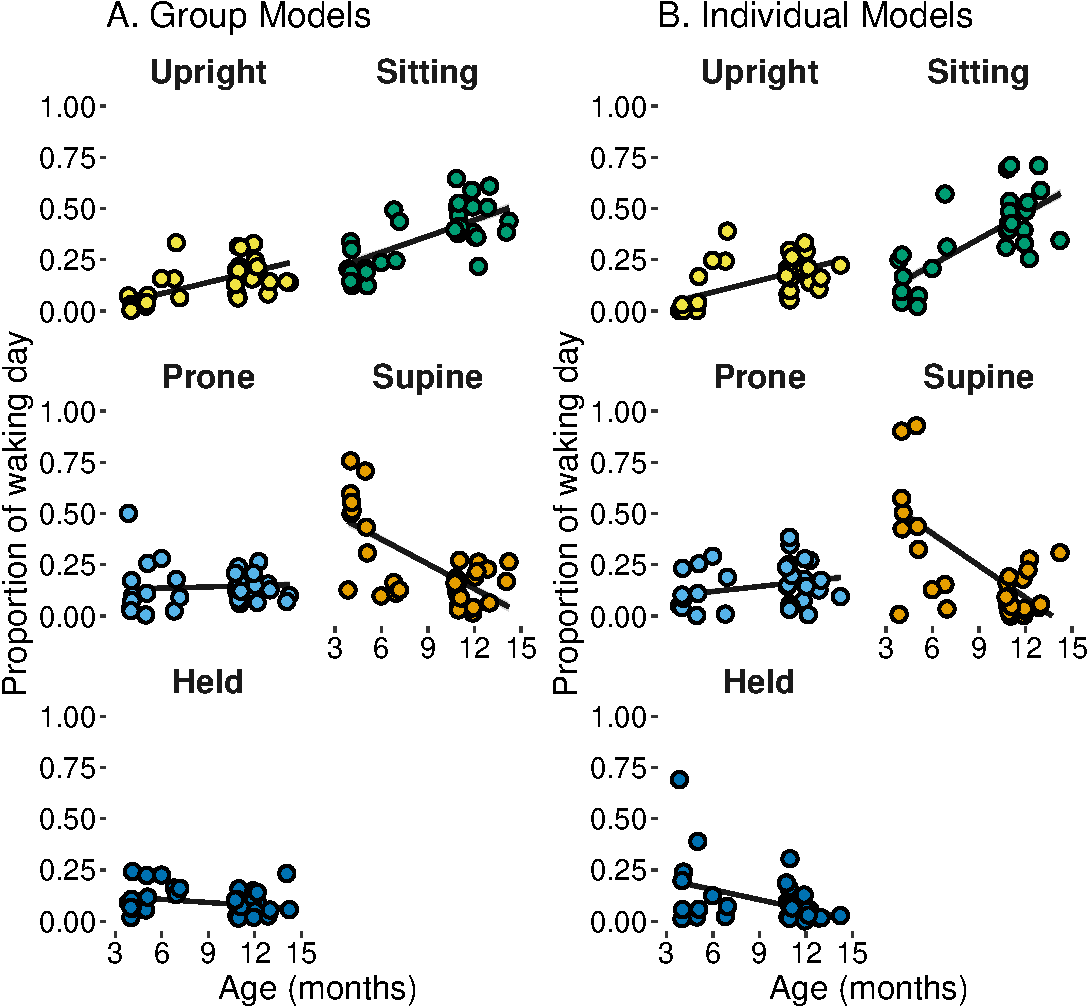
\includegraphics{manuscript_files/figure-latex/age-1} 

}

\caption{Age differences in daily body position predicted from (A) group models and (B) individual models. Each circle represents one full-day recording session's proportion of time in each body position (y-axis) against age in months (x-axis). Black lines indicate best fit regression lines indicating decreases in supine time and increases in sitting and upright time with age.}\label{fig:age}
\end{figure}

\begin{table}[tbp]

\begin{center}
\begin{threeparttable}

\caption{\label{tab:agetable}Summary of age differences in full-day body position for younger (4- to 7-month) and older (11- to 14-month) infants. Values shown are the mean percent of time for each body position averaged across infants in each group. Standard deviations are shown in parentheses. Descriptive statistics are shown separately for group and individual models.}

\begin{tabular}{lllll}
\toprule
 & \multicolumn{2}{c}{Group} & \multicolumn{2}{c}{Individual} \\
\cmidrule(r){2-3} \cmidrule(r){4-5}
Position & Younger & Older & Younger & Older\\
\midrule
Supine & 38.6\% (24.1) & 14.0\% (8.1) & 43.1\% (32.0) & 10.5\% (9.6)\\
Prone & 14.0\% (14.0) & 15.1\% (6.3) & 11.1\% (11.4) & 16.6\% (10.2)\\
Sitting & 28.9\% (15.1) & 44.4\% (9.4) & 20.3\% (14.8) & 46.6\% (12.4)\\
Upright & 5.4\% (7.1) & 18.2\% (7.4) & 9.5\% (13.3) & 18.4\% (7.8)\\
Held & 13.0\% (7.7) & 8.3\% (5.2) & 16.0\% (20.1) & 8.0\% (7.6)\\
\bottomrule
\end{tabular}

\end{threeparttable}
\end{center}

\end{table}

\hypertarget{can-full-day-estimates-of-body-position-reveal-age-differences}{%
\subsubsection{Can Full-Day Estimates of Body Position Reveal Age Differences?}\label{can-full-day-estimates-of-body-position-reveal-age-differences}}

In order to show the convergent validity of the classification method, we demonstrate how the full-day recordings can reveal individual differences in body position according to age, replicating age differences revealed in past work \autocite{Survey}. Table \ref{tab:agetable} summarizes the percent of time that younger and older infants spent in each body position out of their awake samples, as predicted by group and individual models. EMA surveys \autocite{Survey} found that from 3-12 months, infants spent less time held, reclined, and supine but spent increasingly more time sitting and upright. The most straightforward comparisons between the two investigations are upright and prone, because they were defined identically. In \textcite{Survey}, upright time was 0.6-5.5\% of the time for infants 3-6 months, increasing to 22.0\% at 12 months. Results from the current study were similar: younger infants' upright time estimated from full-day group models was 5.41\% compared with 18.24\% for the older group. In \textcite{Survey}, prone time was 2.9-9.2\% of the time for infants 3-6 months, and was 7.2\% at 12 months. In the current study, prone time was 14.03\% for younger infants and 15.09\% for older infants. Furthermore, our results are similar in showing that held and supine time was less for older infants than younger infants (Table \ref{tab:agetable}). Sitting was greater for older infants (44.39\%) compared with younger infants (28.91\%). Moreover, sitting was the most frequent body position followed by upright in 12-month-olds \autocite{Survey}, just as we observed in the current study.

Figure \ref{fig:age} shows that both group and individual model predictions captured age-related differences in body position. Age in months and upright time were significantly, positively correlated using group (\emph{r} = 0.65, \emph{p} \textless{} .001) and individual models (\emph{r} = 0.52, \emph{p} = .002). Similarly, age predicted increases in sitting time using group (\emph{r} = 0.57, \emph{p} \textless{} .001) and individual models (\emph{r} = 0.72, \emph{p} \textless{} .001). In contrast, age predicted decreases in supine time using group (\emph{r} = -0.61, \emph{p} \textless{} .001) and individual models (\emph{r} = -0.61, \emph{p} \textless{} .001). No clear age trends were found for prone time. Age was not significantly related to held time for group models (\emph{r} = -0.25, \emph{p} = .148), but individual models showed a significant negative correlation (\emph{r} = -0.37, \emph{p} = .039) resulting from an outlier in the younger group.

\hypertarget{discussion}{%
\section{Discussion}\label{discussion}}

Here, we demonstrated the validity of long-form recordings of infant body position using wearable inertial sensors. Models trained during the proximal comparison period performed well on testing data collected from the same recording period. Most important, accuracy was consistently strong later in the recording when behavior was completely unsupervised: Human-coded and model-predicted durations of body positions during the distal comparison period were highly correlated, even when narrowing to the scale of 10 minutes. Examining full recordings showed that the new method allows us to capture more data (median = 6.14 hours of awake behavior) than is typical with video methods (1-2 hours) while simultaneously reducing the human labor needed to annotate it. Ultimately, age differences in body position mirrored past findings that employed other methods, suggesting that the outcome of full-day body position recordings is suitable for describing developmental changes in motor behavior.

\hypertarget{accurate-results-in-challenging-circumstances}{%
\subsection{Accurate Results in Challenging Circumstances}\label{accurate-results-in-challenging-circumstances}}

How did classification in the current investigation compare to prior work \autocite{FranchakScott2021,AiraksinenRasanen2020,AiraksinenGallen2022}? Across body positions, median accuracy was 89.40\% for group models (Kappa = 0.77) and 93.30\% for individual models (Kappa = 0.85) during the proximal comparison. Although these accuracy and kappa values are slightly lower than in past work (accuracy 95-98\%, kappas .93-.95), we note that those past values were obtained under ideal circumstances. A researcher applied the sensors in the lab \autocite{FranchakScott2021,AiraksinenRasanen2020} or home \autocite{AiraksinenGallen2022} and set the stage for how infants and caregivers should interact. For example, both \textcite{FranchakScott2021} and \textcite{AiraksinenGallen2022} instructed the caregivers that the recorded sessions should mimic ``playtime'', which would encourage more common activities that would be easier to classify (e.g., crawling and sitting on the floor) and discourage idiosyncratic and potentially more challenging activities (e.g., positioning in infant-specific furniture like exersaucers and walkers, sitting or lying for long periods while eating or nursing). Examining the timelines in Figure \ref{fig:timelines} shows how much variability there is between and within sessions in the earlier parts of the recording that were used for training and testing.

The challenge increased in the distal comparison period. Since sessions were scheduled at convenient times for the infant and caregiver, the transition from the proximal to distal period increased the odds that infants might need a nap, a snack/meal, or engage in a less typical activity (e.g., watching TV). Indeed, the distal comparison in Figure \ref{fig:exemplar-timeline} contains a long period (almost 50 minutes) where the infant sat in a high chair eating lunch. Regardless of these challenges, accuracy in the distal comparison continued to be strong. Barring two outliers (which we will discuss further), agreement was high for group (\emph{r} = 0.92) and individual models (\emph{r} = 0.94). Even at a finer timescale, most errors within 10-minute bins were less than 1 minute in total for all five body positions. For comparison, the reliability of human coders on the body position code was \textasciitilde90\%, putting model-predicted accuracy on a similar level to human coders.

Idiosyncrasies in activities and device use make it challenging to decide \emph{a priori} whether ``odd'' classifications (from the expectation of the researcher) are possible. For example, younger infant \#8 on Figure \ref{fig:timelines} spent an unusual amount of time upright at an age where infants cannot yet stand. Inspecting the video revealed that the infant spent long periods of time suspended in a jumper that supported their body in an upright position. Although it is not feasible to collect large amounts of video data to check model predictions, interviewing caregivers about common activities and devices may provide a way to understand unexpected predictions. Counterintuitively, the two outlier participants increased our confidence that the body position classification method works as intended. At first glance, seeing low agreement rates for two sessions would suggest that the models perform poorly at predicting some \emph{infants'} behavior. Instead, we found that for those infants, errors were restricted to two positions during a single, long-lasting event, while the other three body positions continued to be classified correctly. In other words, the models failed to predict a particular \emph{event} for each of the two infants.

\hypertarget{benefits-and-drawbacks-of-different-modeling-approaches}{%
\subsection{Benefits and Drawbacks of Different Modeling Approaches}\label{benefits-and-drawbacks-of-different-modeling-approaches}}

Throughout the paper, we compared results from two modeling approaches: group models that included all participants' data in the training set versus individual models that used only one participant's data. When considering different metrics, testing periods, body positions, as well as the logistical benefits of each, there is no clear winner. Below, we discuss the pros and cons to each approach so that researchers might decide what works best for their intended application.

Overall accuracy and kappa values were better in individual models compared with group models when collapsed across body positions in the proximal period. However, within-class performance did not always favor individual models---prone predictions were better for group models, and held predictions were almost identical. In the distal comparison (after removing outliers), overall correlations were nearly identical. Within classes, group models had an advantage for prone, upright, and held, whereas individual models had an advantage for sitting and supine. Possibly, individual models are better suited for capturing unique aspects of the devices used for sitting and reclining that lead to better performance in those classes. Finally, age effects (either by group or by age correlation) were nearly identical across the two methods, suggesting that either method would lead to the correct conclusion regarding developmental changes in body position. Outliers were present in both models' predictions: group models produced three sessions with the worst overall accuracy, but individual models produced the single worst kappa. The outliers for the distal comparison period appeared in both models' predictions. For aggregated full-day body position, the most blatant outlier (a young infant held \textgreater{} 60\% of the day) resulted from an individual model. The choice of model might depend on which behavior is most important to capture for a given research question.

Aside from differences in validity, researchers may favor one modeling approach based on logistical concerns. Group models have several major advantages. First, by definition they are trained on more data, which might make predictions more consistent. Second, group models remove the need to get optimal training data from each participant. It can be difficult to elicit every behavior of interest in each infant; individual models require that every behavior that will be later predicted was displayed by each individual infant. In fact, group models remove the need to get \emph{any} training data for a particular infant. Finally, applying a group model means that individual differences between infants are due to their behavior being classified in a consistent way, rather than having a separate set of rules for predicting each individual. However, given the variety in infant behavior, individual models are more agile in capturing the unique and unexpected. Likewise, individual models can be an excellent choice for rapid prototyping and pilot testing. A researcher can get proof-of-concept data from a single participant or a new kind of classification scheme (i.e., locomotion, restraint in device) without annotating an entire sample. Individual models may also be applied in clinical cases where infants vary widely in their motor abilities and/or use of assistive devices.

As in past work \autocite{AiraksinenRasanen2020}, performance was best when using all four sensors and degraded when using any subset of two (i.e., thighs only, left leg only). Small decrements and accuracy were seen for some pairs (particularly when using the left ankle and thigh), but decrements for other pairs (both ankles) or individual sensors were substantial. Using a thigh and ankle pair instead of four sensors would be more cost effective without a large decrease in accuracy, but in some applications the increased accuracy might be worth the cost. Beyond group and individual models and sensor pairings, there were many degrees of freedom in our choice of how best to model body position. For the sake of brevity, we chose to report the best approach, not every possible variation in modeling. However, our openly shared data and code allow researcher to experiment with different sets of motion features, different sets of training data, different machine learning algorithms, and different hyperparameter values. We tested but did not report models that used either only accelerometer data and only gyroscope data; in both cases, performance was degraded compared with models that use both types of motion. We also tried different machine learning algorithms (XGBoost, Tabnet), but found that random forest models performed the best. Finally, we tried modeling each age group separately, but found no benefit to performance by tailoring to the particular age group.

\hypertarget{novel-research-possibilities}{%
\subsection{Novel Research Possibilities}\label{novel-research-possibilities}}

Long-form recordings of motor behavior bring about new research possibilities. Although past work using video \autocite{Karasik2011,ChenSchneider2022,HerzbergFletcher2021} produced real-time data, such data were limited to a relatively small part of the infants' day. And although survey methods \autocite{Survey} could capture moments scattered throughout the day, they do not produce real-time data. The combination of real-time, full-day data about infant motor behavior is unprecedented and offers new opportunities for understanding infants' everyday experiences. Collecting dense data over the entire variety of daily experiences helps to more accurately measure infants' experiences in aggregate (as in Figure \ref{fig:age}) without biasing results from a particular type of activity (e.g., play). Long-form recordings also have the potential to measure clinically-relevant outcomes for infants with motor delay or other pediatric concerns.

In the past decade, developmental scientists have discovered that distributional information about infants' experiences matter for how infants learn \autocite{ClerkinHart2017,KachergisYu2017,RazAbney2019}. Skewed distributions---those that favor the repetition of a small subset of experiences---facilitate learning. For example, recordings from wearable head cameras in the home indicate that infants see a small subset of objects with high frequency \autocite{ClerkinHart2017}, but most objects are seen infrequently. Heterogeneity is also found in how experiences are distributed in time---burstiness and clustering are seen in infants' daily experiences seeing objects and hearing music \autocite{MendozaFausey2022,CasillasElliott2021}. Long-form motor recordings provide a novel opportunity to measure the temporal structure in the sequences of body positions seen in Figure \ref{fig:timelines}. How skewed are infants' experiences with different motor behaviors, and how are they clustered in time? Linking the distributional structure of a particular motor experience in a real day, such as time spent sitting, might be predicted by sitting skill and/or might predict infants' future sitting ability. Moreover, real-time recording of motor behavior provides a way to measure how infant motor behavior links to other types of experiences in the moment in daily life.@MalachowskiSalo2023 used a combination of LENA® and EMA surveys to find that infants heard less adult speech when restrained in seating devices. Combining LENA® and long-form motor recordings can take this a step further by measuring more precisely how speech and body position co-vary within a day.

What underpins these novel research applications is that body position classifications can be applied automatically at scale. Annotating a video corpus of infant behavior from a moderately sized sample---such as 40 infants recorded for 2 hours each in 2 separate visits \autocite{HerzbergFletcher2021}---is incredibly labor intensive. Annotating a larger, more representative sample of \emph{hundreds of infants} while simultaneously scoring \emph{full-day data} would be prohibitive. With sufficiently accurate group models, researchers could annotate a moderately-sized video corpus to then apply the model to hundreds of full-day recordings. Unlike with video, the added cost of more IMU sensor recording time is low, meaning that future studies could sample across multiple days of behavior to better understand intra- versus inter-day variability. Prior diary methods show that infants inconsistently display new motor skills on a day-to-day basis \autocite{AdolphRobinson2008,AdolphRobinson2011}. Multi-day recordings could further uncover how infants' experiences vary over timescales from seconds to days.

\hypertarget{limitations}{%
\subsection{Limitations}\label{limitations}}

We acknowledge several limitations in the current approach. First, a stronger test of full-day accuracy would be to compare accuracy at the start of the recording period to accuracy at the end, rather than using the distal comparison video that followed the first 90 minutes of the study. As we described in the procedure section, synchronizing video cameras and inertial sensors required capturing a synchronization point on video. We completed this procedure prior to giving equipment to caregivers so that they were not responsible for synchronization; in fact, caregivers never (purposefully) touched a button on the video camera. An end-of-day video would require a lot of effort and compliance on the part of caregivers, and any mistakes in the procedure would lead to misaligned and unusable data. Given that most recordings ended at infants' bedtimes, having an experimenter visit families in the evening to video record would be intrusive.

Second, we relied on caregiver logs of infants' naps and times when sensors were removed to separate usable data (times when infants wore the sensors while awake) from unusable data. Future work should aim to further assess caregivers' perceptions about the usability and comfort of the garment. Although infants wore the sensor garment throughout all of the desired times, we did not collect independent data (aside from caregivers' logs) to verify wear time. Most caregivers were diligent about completing logs, however, there were a few cases that caregivers may have failed to report naps (younger infants \#1 and \#4). In the future, algorithms can be developed to automatically identify periods of sleep and times when sensors are off the body. Such algorithms exist for adults using wrist-worn sensors, however, we did not use them because they have not been validated for infant participants wearing sensors on thighs/ankles. Differences in infants' positioning while asleep (held in caregivers arms, laying in cribs, reclined in strollers and carseats) might make classifying sleep more difficult compared with adults based on movement.

Third, although the goal was to collect fully naturalistic behavior, our recording protocol led to some changes that might have affected (or missed) some behaviors. We opted to restrict recording to times when participants were in the home. Inertial sensors can travel with participants, and there is no doubt that infants could have worn the sensors out of the home on errands. However, we do not yet have training data to detect periods of transportation (e.g., moving in a car or in a stroller) that might add noise and/or lead to misclassification of body positions. It is also unknown whether participants might have behaved differently had they not worn the sensors. The added bulk in the garment from the sensors (including the LENA® recorder) might have made some positions more uncomfortable, such as lying prone with the LENA® recorder worn on the chest, and/or influenced how caregivers chose to position infants throughout the day.

\hypertarget{conclusions}{%
\subsection{Conclusions}\label{conclusions}}

In summary, the current study demonstrates the validity of long-form recordings of infant motor behavior in the home. Our analyses show that body position classifications---whether infants are supine, prone, sitting, upright, or held---are accurate immediately and even following a substantial delay. Most important, we find substantial agreement between human-coded and model-predicted body position for data collected during truly everyday, unsupervised activities that create the most challenging cases for automatic classification. In most cases, model prediction accuracy approached human reliability, suggesting that model predictions can be confidently used in analyses of full-day infant behavior. Examining the resulting corpus of \textgreater{} 200 hours of real-time infant body position showed the feasibility of capturing data covering the majority of infants' awake time and the variety of activities contained therein. A rudimentary analysis of aggregated data showed that full-day position estimates conformed to expectations about age differences in motor behavior. Future work employing the method can go beyond aggregated measures of behavior to uncover the temporal structure in infants' daily motor experiences.

\newpage

\hypertarget{declarations}{%
\section{Declarations}\label{declarations}}

\hypertarget{funding}{%
\subsection{Funding}\label{funding}}

This work was funded by National Science Foundation Grant BCS \#1941449.

\hypertarget{competing-interests}{%
\subsection{Competing Interests}\label{competing-interests}}

The authors have no competing interests to declare that are relevant to the content of this article.

\hypertarget{ethics-approval}{%
\subsection{Ethics Approval}\label{ethics-approval}}

The study was performed in accordance with the ethical standards as laid down in the 1964 Declaration of Helsinki. The study procedures were approved by the Institutional Review Board of the University of California, Riverside, Protocol HS-15-050.

\hypertarget{consent}{%
\subsection{Consent}\label{consent}}

Consent to participate: All caregivers provided written informed consent prior to the start of the study.
Consent to publish: Additional written consent was obtained by caregivers for data sharing of audio and video data.

\hypertarget{data-material-and-code-availability}{%
\subsection{Data, Material and Code availability}\label{data-material-and-code-availability}}

A Databrary repository (\url{https://nyu.databrary.org/volume/1580}) includes an exemplar participant's recording session, with the raw video data files, the Datavyu annotations of those video files, a log file with machine-readable synchronization points and nap/diaper change times, and accelerometer and gyroscope data for each of the 4 sensors. A GitHub repository (\url{https://github.com/JohnFranchak/body_position_classification_example}) contains the exemplar participant's data and source code to: 1) synchronize IMU and video annotations, 2) calculate windowed motion features for their data, and 3) train and test the body position classifier using an ``individual model''. Because of the overall size of the full dataset and the computational power/time required to synchronize and create windowed datasets for each session, it would not be feasible to reproduce the calculations for all 34 sessions. However, in a second Github repository (\url{https://github.com/JohnFranchak/body_position_classification_ms}) we share the full results of those computations: The dataset of windowed motion features with corresponding body position codes used to validate the method.

\newpage

\hypertarget{references}{%
\section{References}\label{references}}

\hypertarget{refs}{}
\begin{CSLReferences}{0}{0}
\end{CSLReferences}


\printbibliography

\end{document}
